\documentclass[a4paper,12pt]{article}
\usepackage[utf8]{inputenc}
\usepackage{amsmath, amssymb, amsthm, float, pdflscape, graphicx, pgfplots, tikz, forest, xcolor, lstlinebgrd, mdframed}
\usepackage{lmodern, caption} 
\usepackage[T1]{fontenc}
\usepackage[german]{babel}  
\usepackage{csquotes} 
\usepackage[margin=2.5cm]{geometry}
\usepackage{marginnote}
\usepackage{listings}
\usepackage[most]{tcolorbox}
\usetikzlibrary{trees}
\tcbuselibrary{listings,skins}
% \usepackage[a4paper, top=2cm, bottom=2cm, left=3cm, right=3cm, marginparwidth = 1.75cm]{geometry}

% \usepackage[onehalfspacing]{setspace}
%   \renewcommand{\baselinestretch}{1.55}
\newcommand{\markstep}[2]{\colorbox{marker}{#1}\marginnote{\textbf{(#2)}}}

\tcbuselibrary{listings,skins}

\pgfplotsset{compat=1.18}

\captionsetup[figure]{labelformat=empty}

\newtheorem{theorem}{Theorem}[section]
\newtheorem{lemma}[theorem]{Lemma}
\newtheorem{corollary}[theorem]{Korollar}
\allowdisplaybreaks


\theoremstyle{definition}
\newtheorem{definition}[theorem]{Definition}

\theoremstyle{remark}
\newtheorem*{remark}{Bemerkung}

\forestset{
  fft tree/.style={
    for tree={
      align=center,
      parent anchor=south,
      child anchor=north,
      edge={thick},
      l sep=10mm,
      s sep=2mm,
      inner sep=1pt,
      rounded corners=2pt,
      draw,
      minimum width=16mm,
      font=\scriptsize
    }
  }
}

\definecolor{marker1}{RGB}{255, 255, 128} % Gelb
\definecolor{marker2}{RGB}{144, 238, 144} % Hellgrün
\definecolor{marker3}{RGB}{173, 216, 230} % Hellblau

\lstdefinelanguage{C++}{
  language=C++,
  moredelim=**[is][\markerA]{`}{`}
}

\lstset{
  language=C++,
  basicstyle=\ttfamily\small,
  keywordstyle=\color{blue},
  commentstyle=\color{gray},
  stringstyle=\color{red},
  columns=fullflexible,
  numbers=left,
  numberstyle=\tiny,
  stepnumber=1,
  breaklines=true,
  keepspaces=true,
  breakatwhitespace=true,
  showstringspaces=false,
  framexrightmargin=2pt,
  frame=single,
  tabsize=4,
  escapeinside={(*@}{@*)},
  moredelim=[is][\color{yellow}]{@y@}{@y@},       % rot
  moredelim=[is][\color{blue}]{|b|}{|b|},      % blau
  moredelim=[is][\color{green}]{@g@}{@g@},
  literate={Ä}{{\"A}}1 {Ö}{{\"O}}1 {Ü}{{\"U}}1
           {ä}{{\"a}}1 {ö}{{\"o}}1 {ü}{{\"u}}1 {ß}{{\ss}}1 
           literate={\{}{{\{}}1 {\}}{{\}}}1
           {1)}{{\textcolor{green}{1)}}}1
           {2)}{{\textcolor{yellow}{2)}}}1
           {3)}{{\textcolor{blue}{3)}}}1
}

\lstdefinestyle{mystyle}{ 
  language=C++, 
  basicstyle=\ttfamily\small, 
  keywordstyle=\color{blue}, 
  commentstyle=\color{gray}, 
  stringstyle=\color{red}, 
  columns=fullflexible, 
  numbers=left, 
  numberstyle=\tiny, 
  stepnumber=1, 
  breaklines=true, 
  keepspaces=true, 
  breakatwhitespace=true, 
  showstringspaces=false, 
  frame=single, 
  tabsize=2, 
  literate={Ä}{{\"A}}1 {Ö}{{\"O}}1 {Ü}{{\"U}}1 {ä}{{\"a}}1 {ö}{{\"o}}1 {ü}{{\"u}}1 {ß}{{\ss}}1
}


\title{Fourier-Methoden: Theorie und Anwendungen}
\author{Felix Wager}
\date{\today}



\begin{document}

\thispagestyle{empty}
\begin{center}

\vspace*{1cm}

\begin{tabular}{p{7cm}p{7cm}}
\textbf{Willibald-Gluck-Gymnasium} & \hfill \textbf{Oberstufenjahrgang 2024/26} \\
Neumarkt in der Oberpfalz & \\
\end{tabular}

\vspace{3cm}

\textbf{\Large S E M I N A R A R B E I T}\\[0.3cm]
aus dem W-Seminar\\[0.3cm]
\textit{„Mathematik ist überall“}

\vspace{2cm}
\begin{flushleft}
Thema der Seminararbeit:
\end{flushleft}
\begin{center}
\textbf{Analysis:}\\
Die Fouriertransformation ...
\end{center}

\vspace{2cm}

\begin{flushleft}
\textbf{Verfasser:} \hspace{2cm} Felix Wager\\[0.3cm]
\textbf{Kursleiter:} \hspace{2.5cm} OSR Albert Thumann\\[0.3cm]
\textbf{Abgabetermin:} \hspace{1.6cm} 11.\ November\ 2025
\end{flushleft}

\vspace{2cm}

\begin{flushleft}
\begin{tabular}{@{}l l l l@{}}
\textbf{Bewertung der schriftlichen Arbeit:} & \rule{1cm}{0.4pt} & Punkte & in Worten: \rule{3cm}{0.4pt} \\[0.4cm]
\textbf{Bewertung der Präsentation:} & \rule{1cm}{0.4pt} & Punkte & in Worten: \rule{3cm}{0.4pt} \\[0.4cm]
\textbf{Gesamtbewertung} ($\frac{3 \; \cdot \text{ schriftlich } + \; 1 \; \cdot \text{ mündlich}}{2}$): & \rule{1cm}{0.4pt} & Punkte & \\
\end{tabular}

\vspace{0.8cm}

\textbf{Abgabe bei der Oberstufenkoordinatorin am:} 11.\ November\ 2025
\end{flushleft}

\vfill

\begin{flushright}
\rule{5cm}{0.4pt}\\
Unterschrift des Kursleiters
\end{flushright}

\end{center}

\renewcommand{\contentsname}{Inhaltsverzeichnis}
\tableofcontents

\section{Abstract}

\section{Einleitung}
\subsection{Motivation}
Warum Fourier-Methoden heute so wichtig sind.
\subsection{Zielsetzung der Arbeit}
\subsection{Aufbau der Arbeit}

\section{Mathematische Grundlagen}
\subsection{Komplexe Zahlen und die Eulerformel}
Um sich die Arbeit mit Fourier Transformationen, Reihen und sonstigem erheblich zu erleichtern ist es sehr sinnvoll mit komplexen Zahlen zu arbeiten. Doch was sind komplexe Zahlen? 
Komplexe Zahlen sind prinzipiell nichts anderes, als eine Erweiterung der Menge der Reellen Zahlen, welche es ermöglicht die Wurzel von negativen Zahlen zu ziehen. Dafür wird die Wurzel von $-1$ als die imaginäre Einheit $i$ definiert. Mathematisch korrekt sieht das wie folgt aus:
$$i^2 := -1$$
Die Menge der komplexen Zahlen wird mit dem Symbol $\mathbb{C}$ abgekürzt. Eine typische komplexe Zahl hat in der algebraischen Schreibweise die Form:
$$ z = a + ib \quad \text{mit} \quad a,b \in \mathbb{R} $$
$a$ ist hierbei der Realteil $\Re(z)$ und $b$ der Imaginärteil $\Im(z)$ von $z$. \vspace{1em}

Um mit komplexen Zahlen bei Fourier Reihen zu arbeiten, benötigt man auch ein paar Rechenoperationen. Die wichtigsten beiden sind hier der Betrag und das komplex konjugierte einer komplexen Zahl. Eine komplexe Zahl lässt sich auch als Vektor im $\mathbb{R}^2$ betrachtet, so ist dann der Betrag als euklidische Norm dieses Vektors definiert. 
$$\vert{z}\vert := \|z\| = \sqrt{ a^2 + b^2}$$
Bedeutet in einem Koordinatensystem, bei dem der Real- und Imaginärteil einer Zahl auf den x- und y-Achsen festgehalten wird, ist der Betrag die Länge vom Ursprung bis zum Punkt im Koordinatensystem dieser Zahl. 
Und das komplex konjugierte einer Zahl ist eine Abbildung, welche lediglich den Imaginärteil mit $-1$ multipliziert:

$$\bar{}\;:\mathbb{C}\;\to\mathbb{C},\; z = x+iy \mapsto \bar{z} := x-iy$$

Mithilfe von komplexen Zahlen und den Taylorreihen von Sinus, Cosinus und der Exponentialfunktion $e^x$ kann man nun die Eulerformel herleiten. 

 $$e^{ix} = \cos{x} + i\sin{x}$$

Wenn man den Betrag dieses Ausdrucks bildet, so fällt auf, dass hier das Ergebnis, unabhängig von $x$, 1 ist. Dies bedeutet, dass $e^{ix}$ als ein gegen den Uhrzeigersinn rotierender Vektor, für steigende Werte für $x$, gesehen werden kann. Im vorher genannten Koordinatensystem, welches man auch die Gaußsche Zahlenebene nennt, sieht das so aus:
\begin{center}
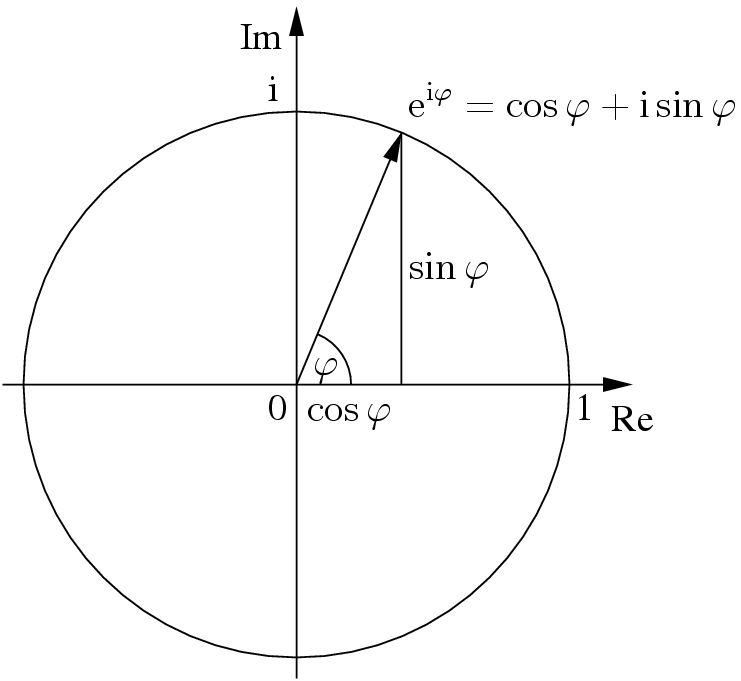
\includegraphics[scale=0.75]{Bilder/eulerformel.jpg}
\end{center}

\subsection{Das Skalarprodukt von Funktionen und Orthonormalsysteme}
Des Weiteren spielen Orthonormalsysteme eine große Rolle, wenn man sich mit der Fourier Analyse beschäftigt. 
Allgemein lässt sich sagen, dass ein Orthonormalsystem eine Menge von Vektoren oder Funktionen, aus einem Vektorraum mit Skalarprodukt, 
sind, welche sowohl orthogonal zueinander, aber auch normiert zu sich selbst sind. 
Orthogonal sind sie, wenn das Skalarprodukt zweier unterschiedlicher Vektoren 0 ergibt und normiert, wenn das Skalarprodukt eines Vektors mit sich selbst 1 ergibt.
Für alle Vektoren $v_n$ im $\mathbb{R}^n$ muss also folgendes gelten, damit die Menge der Vektoren ein Orthonormalsystem bildet: 
$$\text{1. Orthogonalität: } \langle v_i, v_j\rangle = 0 \quad \forall \:i \neq j $$
$$\text{2. Normiertheit: } \langle v_i, v_j\rangle = \sum_{i=1}^{n}v_i^2 = \|v_i\|^2 = 1 \quad \text{mit} \: i = j$$
$$\left( \text{Skalarprodukt: } \langle v, w\rangle := \sum_{i = 1}^{n}v_i * w_i\right)$$
Hier sieht man auch, dass das Skalarprodukt eines Vektors mit sich selbst, das gleiche 
ist wie die quadrierte euklidische Norm des Vektors, wodurch der Begriff der Normiertheit 
anschaulicher wird. Wie schon erwähnt lassen sich diese Eigenschaften auch auf Funktionen anwenden. 
Hierfür definiert man die Normiertheit und die Orthogonalität auch, exakt gleich wie bei Vektoren, über das Skalarprodukt. Das Skalarprodukt für zwei Funktionen ist wie folgt definiert:
$$\langle v, w \rangle := \int_a^bv{(x)*w(x)dx} \quad \text{für} \: v,w : [a,b] \to \mathbb{R} $$
Falls eine Menge von Funktionen Orthogonalität und Normiertheit erfüllt, ist diese Menge auch ein Orthogonalsystem. 
Anschaulich kann man sich die Funktionen v(x) und w(x) noch als zwei Vektoren mit unendlich 
vielen Dimensionen vorstellen, wobei der x Wert angibt in welcher Dimension man sich befindet. 
Da das Skalarprodukt die jeweiligen Dimensionen von Vektoren multipliziert und diese 
schließlich aufsummiert, macht es Sinn, dass man bei Funktionen ähnlich vorgeht. 
So lässt sich also die Erweiterung der Summe zum Integral erklären.  Die Formel für die 
Norm von Funktionen $\left( \|f\| = \sqrt{\int_a^b{\vert f(x)\vert^2 dx}} \right)$ ergibt sich, wenn man das für Funktionen definierte Skalarprodukt 
ähnlich wie bei Vektoren auf die Funktion selbst anwendet. Im komplexen Fall wird das Skalarprodukt leicht angepasst, 
indem der zweite Faktor komplex konjugiert wird:
$$\langle v,w \rangle := \int_a^b{v(x)*\overline{w(x)}dx} \quad \text{für} \: v,w : [a,b] \to \mathbb{C}$$

\subsection{Die Fourierreihe}
Der erste große Schritt, um die Fourier Transformation herzuleiten, ist die Fourier Reihe. 
Eine Reihe selbst ist in der Mathematik ist ein Begriff für eine unendliche Summe von Termen. 
Die Fourier Reihe ist hierbei eine besondere Reihe. Ihr Sinn ist es periodische Funktionen 
mithilfe von Sinus- und Kosinustermen zu approximieren.  Joseph Fourier hat in seinem Werk 
„Théorie analytique de la chaleur“ schließlich auch beweisen, dass jede periodische Funktion 
auf diese Weise dargestellt werden kann. Die Approximation selbst geschieht durch 
trigonometrische Polynome, mit welchen man später die Fourierreihe einer Funktion bildet. 
Ein trigonometrisches Polynom ist hier eine Funktion der Form: 
$$p(x) = a_0 + \sum_{k=1}^n{a_k \cos(kx) + b_k \sin(kx)}  \quad a_k,b_k \in \mathbb{R}$$
Ziel ist es nun die Faktoren $a_k$ und $b_k$ in Abhängigkeit zur anzunähernden Funktion zu 
bestimmen. Denn durch die Zählervariable k, welche die Periodenlänge der Sinus- und 
Kosinusterme bestimmt, kann man durch die Faktoren $a_k$ und $b_k$ festlegen wie dominant 
die Anteile der Sinus und Kosinusterme, mit der jeweiligen Periodenlänge, in der zu 
approximierende Funktion sind. Um die Berechnung der Faktoren kompakter zu gestalten, 
kann man mit dem Zusammenhang $2\cos{x} = e^{ix} -e^{-ix}$ und $2i\sin{x} = e^{ix}+e^{-ix}$, 
einer Umstellung der Eulerformel, nun das trigonometrische Polynom zu dem komplexen 
trigonometrischen Polynom zusammenfassen: 
$$p(x) = \sum_{k=-n}^n{c_k \, e^{ikx}} \quad \text{für geeignete} \: c_k \in \mathbb{C}$$
Um jetzt den komplexen Faktor $c_k$, zunächst für $2\pi$ periodische Funktionen, 
zu berechnen, verwendet man ein Orthonormalsystem, welches aus den Funktionen $\varphi_n(x)$ besteht:
$$\phi_n(x):[-\pi,\pi] \to \mathbb{C}, \quad \phi_n(x) = \frac{1}{\sqrt{2\pi}} \, e^{inx} \quad \text{mit} \: n\in \mathbb{Z}$$
Dass die Menge an Funktionen $\phi_n$ ein Orthonormalsystem ist, habe 
ich im Anhang gezeigt (Beweis A. 1). Um endlich $c_k$ zu berechnen, setzt man zunächst 
die zu approximierende Funktion $f$, mit der Periodizität $2\pi$, mit dem 
trigonometrischen Polynom gleich und schränkt sie zudem ein: 
$$f:[-\pi,\pi]\to \mathbb{C},\quad f(x) = \sqrt{2\pi} * \sum_{k = -n}^n{c_k\phi_k(x)} $$
Anschließend bildet man das Skalarprodukt von $f$ und $\phi_m$, was möglich ist, da 
$f$ auf der Definitionsbereich von $f$ und $\phi_m$ gleich ist. 
$$\langle f, \phi_m \rangle = \int_{-\pi}^\pi {f(x) \overline{\phi_m(x)}dx} = \int_{-\pi}^\pi{\sqrt{2\pi}\sum_{k = -n}^n{c_k\phi_k(x)\overline{\phi_m(x)}}dx}$$
Da Integral und Summe beide linear sind, darf man die Summe mit dem Integral vertauschen. 
Zudem hängt $c_k$ nicht von $x$ ab, wodurch der Faktor $c_k$ für das Integral eine Konstante ist. 
Nach einer Abwandlung des Distributivgesetzes darf er somit herausgezogen werden. Man erhält 
also diesen Ausdruck: 
$$\int_{-\pi}^\pi{f(x)\overline{\phi_m(x)} dx} = \sqrt{2\pi}\sum_{k=-n}^{n}{c_k\int_{-\pi}^\pi{\phi_k(x) \overline{\phi_m(x)} dx}}$$
Aufgrund dessen, dass die Menge der Funktionen $\phi_m$ ein Orthonormalsystem ist, ist jeder Summand, außer $k = m$, 0. Durch die Normiertheit des Orthonormalsystems bleibt übrig:
$$c_m = \frac{1}{\sqrt{2\pi}}\int_{-\pi}^\pi{f(x)\overline{\phi_m(x)}dx} = \frac{1}{2\pi}\int_{-\pi}^\pi{f(x)e^{imx}dx}$$ 

Jetzt ist es möglich mit dieser Formel und dem komplexen trigonometrischem Polynom eine 
$2\pi$ periodische Funktion zu approximieren. Jedoch wäre es hilfreich, wenn dies für alle 
Perioden möglich wäre. Um auch Funktionen mit einer Periodizität von $2L$ annähern zu können, 
muss man den Faktor $c_k$ und das komplexe trigonometrische Polynom auf einer Periodizität von $2L$ ausweiten. 
Damit das trigonometrische Polynom $2L$ periodisch wird muss folgendes gelten: 
$$e^{i\omega x} = e^{i\omega(x+2L)}$$
$\omega$ gilt es dabei herauszufinden, damit das trigonometrische Polynom $2L$ periodisch wird:
$$e^{i\omega x} = e^{i\omega(x+2L)} \Leftrightarrow e^{i\omega 2L} = 1 \Leftrightarrow \omega 2L = 2\pi k \Leftrightarrow \omega_k = \frac{k\pi}{L}$$
Das neue trigonometrische Polynom sieht also so aus:
$$\sum_{k=-n}^n{c_k e^{i\omega_kx}} \Leftrightarrow \sum_{k=-n}^n{c_k e^{i\frac{k\pi}{L}x}}$$
Um $c_k$ zu berechen, nimmt man sich eine $2L$ periodische Funktion $f$ und definiert sich eine $2\pi$ periodische 
Hilfsfunktion $g$ in Abhängigkeit von $f$ wie folgt:
$$g(t) := f\left(\frac{L}{\pi}t\right) $$
Da $g$ eine $2\pi$ periodische Funktion ist, kann man mit der hergeleiteten Formel $c_k$ 
von $g$ berechnen. Um die Formel für $2L$ periodische Funktionen zu erhalten, ist das 
Ziel die Formel über $g$ auf $f$ auszuweiten. Das funktioniert über die Substitutionsregel 
bei Integralen. Um sie anzuwenden, führen wir die Ableitung der inneren Funktion von $f$, 
also $\frac{L}{\pi}$ in Form einer $1$ ein und erhalten die Formel für $c_k$, für die 
Periodizität $2L$: 
$$c_k = \frac{1}{2\pi} \int_{-\pi}^\pi{g(t)e^{-ikt}dt} \Leftrightarrow c_k = \frac{1}{2\pi}*\frac{\pi}{L} \int_{-\pi}^{\pi}{\frac{L}{\pi}f\left(\frac{L}{\pi}t\right)e^{-i\omega_kt} dt}$$
Wendet man jetzt die Substitutionsregel an, erhält man: 
$$c_k = \frac{1}{2L}\int_{-L}^{L}{f(x)e^{-i\omega_kx}dx} = \frac{1}{2L}\int_{-L}^{L}{f(x)e^{-i\frac{k\pi}{L}x}dx}$$

\subsection{Von der Fourierreihe zur Fouriertranformation}
Die Fourierreihe erlaubt es uns, periodische Signale als Summe von Sinus- und Kosinusfunktionen oder komplexen Exponentialfunktionen darzustellen. Doch viele Signale in der Praxis sind nicht-periodisch. Um auch diese Signale in ihre Frequenzanteile zerlegen zu können, verallgemeinern wir das Konzept der Fourierreihe zur Fouriertransformation. Mit der Fouriertransformation werden wir so eine Funktion erhalten, welche uns sagen wird wie groß der Anteil einer Frequenz oder Periodenlänge in einem Signal ist. Dazu nehmen wir die Fourierreihe einer Funktion $f$ mit der Periode $2L$ und der Frequenz $\omega_k$: 
$$f(x) = \sum_{k = -\infty}^{\infty}{c_k e^{i\omega_k x} }, \quad c_k = \frac{1}{2L}\int_{-L}^L{f(x) e^{-i\omega_k x} dx}$$
Dazu definieren wir eine Hilfsfunktion $F(\xi)$: 
$$F:\mathbb{K} \to \mathbb{C}, \quad F(\xi) = \int_{-L}^{L}{f(x) e^{-i \xi x} dx}$$
damit gilt
$$ c_k = \frac{1}{2L} F(\omega_k)$$
Setzt man den neu gewonnen Ausdruck für $c_k$ in die Fourierreihe ein, so erhält man 
$$ f(x) = \sum_{n = -\infty}^{\infty}{F(\omega) e^{i\omega x}}$$
Anschließend bildet man $\Delta \omega$ aus $\omega_k$:
$$\omega_k = k \frac{\pi}{L} \Rightarrow \Delta \omega = \frac{\pi}{L} \Rightarrow \frac{1}{2L} = \frac{\Delta \omega} {2\pi}$$
Und setzt die Gleichung auch in die Fourierreihe ein: 
$$\frac{1}{2\pi} \sum_{k=-\infty}^{\infty}{F(\omega_k) e^{i \omega_k x} \Delta \omega}$$
Dies ist eine Riemann Summe. Lässt man nun $L \to \infty$ laufen, erhält man ein Integral, welches die inverse Fouriertransformation ist:
$$\lim_{L\to\infty} {\frac{1}{2\pi}\sum_{n = -\infty}^\infty{F(\omega_k) e^{i \omega_k x}\Delta \omega}} = \frac {1}{2\pi} \int_{-\infty}^{\infty}{F(\omega)e^{i \omega x} d\omega}$$
Die Funktion $F(\omega)$ selbst ist die Fouriertransformation von $f$:
$$F(\omega) = \int_{-\infty}^{\infty}{f(x) e^{-i\omega x} dx}$$

Man kann das Integral in der Fouriertransformation am besten verstehen, wenn man es 
als eine Art Durchschnitt betrachtet. Ähnlich wie beim Berechnen eines Mittelwerts 
summiert das Integral nicht nur eine endliche Anzahl von Werten auf, sondern unendlich viele, 
unendlich kleine Beiträge von $f(x)$. Im Integral steht dabei das Produkt $f(x) \cdot e^{-i\omega x}$.
Dieses Produkt misst, wie stark die Frequenz $\omega$ in $f(x)$ enthalten ist:
\begin{itemize}
    \item Ist der Anteil der Frequenz $\omega$ in $f(x)$ hoch, dann verstärkt $e^{i\omega_kx}$ den Wert der Funktion $f(x)$
    im Integral konstruktiv und $F(\omega)$ wird groß.
    \item Enthält $f(x)$ diese Frequenz nicht, heben sich die positiven und negativen Anteile 
    im Integral weitgehend auf und $F(\omega)$ wird klein.
  \end{itemize}
So zeigt die Fouriertransformation, wie groß der Anteil jeder einzelnen Frequenz $\omega$ 
in der Funktion $f$ ist.

\subsection{Die Foureirtransformation in der Praxis: Die DFT}
In der Praxis arbeitet man selten mit kontinuierlichen Funktionen, sondern mit diskreten Messwerten, zum Beispiel bei Audiosignalen oder digitalen Bildern. Um diese Signale in ihre Frequenzanteile zu zerlegen, verwendet man die diskrete Fouriertransformation (DFT).
Formell lässt sich die DFT für eine endliche Folge von N Messwerten
$$x_0, x_1,..., x_{N-1}$$
durch die folgende Formel darstellen:
$$X_k = \sum_{j = 0}^{N-1}{x_n e^{-i2\pi \frac{kj}{N}}} \quad \text{mit } k\in[0, N-1]$$
Anzumerken ist aber noch, dass es eine Besonderheit gibt. Wenn das Eingangssignal reell ist, 
liefert die DFT zwar N Koeffizienten, jedoch sind die Frequenzen oberhalb von N/2 wegen des 
Nyquist-Theorems lediglich Spiegelungen der tieferen Frequenzen und enthalten keine neuen 
Informationen. Warum das so ist, werde ich hier nicht näher eingehen. Wie man die Formel für 
die DFT herleitet, erkläre ich im nächsten Kapitel.

\subsection{Die Foureirtransformation in der Praxis: Die FFT}
Obwohl die DFT so in der Praxis anwendbar ist, ist sie heutzutage in fast keinem Programm oder 
Algorithmus zu finden. Denn will man eine Funktion oder Signal mit $N$ Werten komplett 
transformieren, dann muss man für $N$ verschiedene Frequenzen den Wert über die obere Formel 
berechnen. Also sind es insgesamt $N^2$ Berechnungen, die man durchführen muss. In der Informatik 
spricht man für den Abschnitt der DFT in einem Programm von einer Laufzeit von:   $O(N^2)$

Im Jahre 1965 aber, entdeckte James W. Cooley und John W. Tukey eine neue Art die DFT zu 
berechnen, was die Laufzeit auf $O(N\log N)$ verringerte. Somit konnte man die DFT erheblich 
schneller berechnen. Daher kommt auch der Name FFT für den neuen Algorithmus, was für Fast Fourier 
Transform, also schnelle Fouriertransformation, steht. Um die Umformung gut zu sehen, kann man die 
diskrete Fouriertransformation etwas umschreiben. Dafür definiere ich die Folge $(\omega_n)_{n\in\mathbb{N}}$ 
wie folgt:
$$\omega_n := e^{-2\pi i /n}$$
Schreibt man jetzt die Werte der Ausgangsfunktion $f$ als Vektor, kann man aufgrund der Struktur 
der Matrixmultiplikation, diesen Vektor mit einer besonderen Matrix multiplizieren und erhält das 
Ergebnis der Transformation auch in Form eines Vektors derselben Länge, mit den Werten $\hat{f}$. 
\[
\begin{bmatrix}
  \hat{f_0}\\
\hat{f_1}\\
\hat{f_2}\\
\vdots \\
\hat{f_n}\\
\end{bmatrix}
=
\begin{bmatrix}
  1 & 1 & 1 & \cdots & 1\\
  1 & \omega_n & \omega_n^2 & \cdots & \omega_n^{n-1} \\
  1 & \omega_n^2 & \omega_n^4 & \cdots & \omega_n^{2(n-1)}\\
  \vdots & \vdots & \vdots & \ddots & \vdots \\
  1 & \omega_n^{n-1} & \omega_n^{2(n-1)} & \cdots & \omega_n^{(n-1)^2}\\
\end{bmatrix}
\cdot
\begin{bmatrix}
  f_0\\
  f_1\\
  f_2\\
  \vdots\\
  f_n
\end{bmatrix}
\left(
  = 
\begin{bmatrix}
  \omega_n^{0 \cdot 0} & \omega_n^{0 \cdot 1} & \cdots & \omega_n^{0 \cdot (n-1)}\\
  \omega_n^{1 \cdot 0} & \omega_n^{1 \cdot 1} &  \cdots & \omega_n^{1 \cdot (n-1)} \\
  \omega_n^{2 \cdot 0} & \omega_n^{2 \cdot 1} &  \cdots & \omega_n^{2 \cdot (n-1)}\\
  \vdots & \vdots & \ddots & \vdots \\
  \omega_n^{(n-1) \cdot 0} & \omega_n^{(n-1) \cdot 1} & \cdots & \omega_n^{(n-1)^2}\\
\end{bmatrix}
\cdot
\begin{bmatrix}
  f_0\\
  f_1\\
  f_2\\
  \vdots\\
  f_n
\end{bmatrix}
\right)
\]
Jeder Eintrag im Ergebnisvektor entsteht, indem man die Zahlen in der Zeile der Matrix 
mit den Zahlen im Vektor multipliziert und die Produkte zusammenzählt. Deshalb muss 
jeder Eintrag der Matrix aus $\omega_n$ noch mit $k$, der die Frequenz bestimmt, und 
der Zählvariable $j$, die über die Zeilen läuft, als Exponent potenziert werden.

Was Cooley und Tukey herausgefunden haben ist, dass man diesen Ausdruck wie so umschreiben 
kann:

\[\hat{f} = F_N \cdot f = 
\begin{bmatrix}
I_{N/2} & D_{N/2} \\
I_{N/2} & -D_{N/2}
\end{bmatrix}
\cdot 
\begin{bmatrix}
  F_{N/2} & 0 \\
  0 & F_{N/2} \\ 
\end{bmatrix}
\cdot 
\begin{bmatrix}
  f_{gerade} \\
  f_{ungerade}
  \end{bmatrix}
  \]
$F$ ist die DFT-Matrix, mit der der ursprüngliche Wertevektor $f$ multipliziert wurde. 
$I_N$ ist die Einheitsmatrix: Alle Einträge außerhalb der Diagonale sind $0$, auf der 
Diagonale stehen $1$, von links oben nach rechts unten. $D_N$ ist ebenfalls eine Diagonalmatrix 
wie $I_N$, jedoch bestehen die Diagonaleinträge aus $\omega_N^k$, wobei $k$ von $0$ bis $N-1$ 
läuft. Der Index der Matrizen gibt jeweils die Anzahl der Zeilen und Spalten an. $f$ wurde den Indizes nach aufgeteilt. 

Wichtig ist, diese Formel funktioniert nur, wenn die Anzahl der Werte der Ausgangsfunktion 
eine Zweierpotenz ist. Zumal das genau der Grund ist, warum die Umstellung es überhaupt schafft die Laufzeit 
so drastisch zu reduzieren. Das was diese Formel ausmacht sind eigentlich nur die letzen beiden 
Faktoren des Produkts. Denn multipliziert man diese Faktoren miteinander, dann fällt auf, dass 
man diesen Ausdruck erhält:
\[
\begin{bmatrix}
F_{N/2} \cdot f_{gerade} & 0 \\
0 & F_{N/2} \cdot f_{ungerade} 
\end{bmatrix}
\]

Auffällig ist jetzt, dass man zwei mal das Anfangsproblem, in halber Größe erhält. Man könnte 
zunächst denken, dies mache keinen Unterschied, aber dadurch dass die Berechnung der komplette Matrix, einen
Aufwand von $O(N^2)$ erfordert, reduziert man mit jeder Anwendung der Formel die Laufzeit für 
die Berechnung von $F_{N/2} \cdot f$ auf $O((N/2)^2)$. Wendet man diese Formel rekursiv, also 
immer wieder auf sich selbst, an, bis man Matrizen mit einer Größe von 1 oder 2 erhält, so 
schafft man es, durch ein zeitsparendes zusammenfügen, die Laufzeit der Berechnung auf 
$O(N\log N)$ zu kürzen. Die Struktur einer FFT mit 8 Werten, kann man auch so darstellen:
\\ \\ \\
\begin{forest}
  fft tree
  [
    {\(F_8\cdot f_8\)\\(ganze DFT)}
    [
      {\(F_4\cdot f_4\)\\(gerade)}
      [
        {\(F_2\cdot f_2\)\\(gerade)}
        [\(F_1\cdot f_1\)\\(gerade)]
        [\(F_1\cdot f_1\)\\(ungerade)]
        ]
        [
          {\(F_2\cdot f_2\)\\(ungerade)}
          [\(F_1\cdot f_1\)\\(gerade)]
          [\(F_1\cdot f_1\)\\(ungerade)]
          ]
          ]
          [
            {\(F_4\cdot f_4\)\\(ungerade)}
            [
              {\(F_2\cdot f_2\)\\(gerade)}
              [\(F_1\cdot f_1\)\\(gerade)]
              [\(F_1\cdot f_1\)\\(ungerade)]
              ]
              [
                {\(F_2\cdot f_2\)\\(ungerade)}
                [\(F_1\cdot f_1\)\\(gerade)]
                [\(F_1\cdot f_1\)\\(ungerade)]
                ]
                ]
                ]
              \end{forest}
\\ \\ \\ 
In meinem Programm, zu welchem ich im nächsten Kapitel komme, mit welchem ich eine Audiospur 
aufnehme und verarbeite, nutze ich eine auf meinem Gerät eine Samplerate von 44800. Bedeutet 
ich nehme pro Sekunde 44800 Datenpunkte auf. Wenn man nun die Laufzeit einer DFT und einer FFT 
grob skizziert, sieht man, dass bei der Verarbeitung eines Signals, mit nur einer Sekunde, bei 
meinem Programm die DFT mehr als doppelt so lang dauert, wie die FFT.  

\begin{figure}[!h]
\centering
\begin{tikzpicture}
  \begin{axis}[
    width=12cm, height=8cm,
    xlabel={Samples $N$},
    ylabel={Operationen},
    %title={Vergleich der Laufzeit von DFT und FFT},
    axis lines=left,
    clip=false,
    xmin=0, xmax=45000,
    ymode=log,
    legend style={at={(0.02,0.98)},anchor=north west},
    ytick style={draw=none} % nur Striche entfernen
    ]
    % DFT: O(N^2)
    \addplot[blue, thick, samples=200, domain=100:44800] {x^2};
    \addlegendentry{DFT O($N^2$)}
    
    % FFT: O(N log N)
    \addplot[red, thick, samples=200, domain=100:44800] {x*ln(x)/ln(2)};
    \addlegendentry{FFT O($N \log_2 N$)}
  \end{axis}
  \end{tikzpicture}
%\caption{Vergleich der Laufzeit von DFT und FFT für Sample-Größen $N$ bis 44{,}800}
\end{figure}



\section{Von der Theorie zu Praxis: Eigenentwicklung eines Audioanalyzers mit C++}
Nachdem im vorherigen Kapitel die mathematischen Grundlagen der Fouriertransformation und 
ihrer diskreten Varianten vorgestellt wurden, möchte ich nun zeigen, wie ich diese Konzepte 
praktisch umgesetzt habe. Angefangen hat alles mit der Idee einen eigenen Audioanalyzer zu 
programmieren. Dieser soll live ein Audiosignal aufnehmen, dieses Visualisieren und anschließend 
die Frequenzanteile, die in dem Signal enthalten sind, anzeigen. Somit könnte ich mithilfe 
meines eigenen Programms Musik genauer unter die Lupe nehmen, die Funktion der Fouriertransformation 
so manipulieren, dass Rauschen unterdrückt wird, Töne von Tieren oder Instrumenten erkennen 
oder auch Raumresonanzen sichtbar machen. Als ich mit dem Programmieren begann und alles 
zur Liveaufnahme eines Audiosignals implementiert hatte, stieß ich auf eine erste Schwierigkeit. 
Mein Problem war der Übergang von der Theorie der Fouriertransformation zur Praxis. Denn 
ich hatte ein Signal in Form einer Liste von Zahlen, wodurch die normale Formel für die 
Fouriertransformation durch das Integral nicht anwendbar war. Da ich zum damaligen Zeitpunkt 
die diskrete Fouriertransformation nicht kannte, versuchte ich eigenständig eine Approximation 
der Formel für endliche Werte zu finden. Im folgenden Abschnitt zeige ich also, wie ich 
eigenständig die DFT mit einer minimalen Abweichung hergeleitet habe.
\subsection{Eigenständige Herleitung der DFT}
Da ich, wie zuvor erwähnt, die DFT noch nicht kannte, versuchte ich zunächst aus den Punkten, 
also die Daten der Audioaufnahme, eine Funktion zu erstellen, auf welche die Formel anwendbar 
ist. Ein Hauptkriterium, um die Formel zu realisieren ist, dass die Funktion integrierbar ist. 
Natürlich kann man ausgehend von den Punkten viele Rechtecke nutzen und diese als Approximation 
für die Fläche des Integrals zu benutzen. Das sähe so aus:

\begin{figure}[h!]
\centering
\begin{tikzpicture}[>=stealth]

  % Achsen
  \draw[->] (-0.5,0) -- (15.5,0) node[right] {$n$};
  \draw[->] (0,-2.5) -- (0,2.5) node[above] {$f(n)$};
  
  % Winkel pro Einheit (in Grad) sodass 1.5 Perioden auf [0,14] liegen
  \pgfmathsetmacro{\degPerUnit}{180*3/14} % = 38.5714286...
  
  % Diskrete Punkte f(n) (aus der Sinusfunktion)
  \foreach \x in {0,...,14} {
    \pgfmathsetmacro{\yy}{2*sin(\degPerUnit*\x)} % sin erwartet hier Grad
    \fill[red] (\x,\yy) circle (2pt);
    \node[red, above, font=\scriptsize] at (\x,\yy) {$f(\pgfmathprintnumber{\x})$};
    \draw[dashed, gray!60] (\x,0) -- (\x,\yy);
    }
    
    % Rechteckflächen (linke Riemann-Summe)
    \foreach \i in {0,...,13} {
      \pgfmathsetmacro{\y}{2*sin(\degPerUnit*\i)} % Höhe = f(n)
      \fill[blue!20, opacity=0.5] (\i,0) rectangle (\i+1,\y);
      }
      
      % (Optional) kontinuierliche Referenz-Sinuskurve mit gleicher Frequenz
      \draw[domain=0:14, smooth, samples=300, thin, red!70] plot(\x,{2*sin(\degPerUnit*\x)});
      
      % Beschriftung Rechteckformel
      \node at (9,-2.3) {\footnotesize Fläche Rechteck: $A = (x_{n+1}-x_n)\,f(n)$};
      
    \end{tikzpicture}
  \end{figure}
Das Bild zeigt, wie man eine gekrümmte Fläche (die Sinuskurve) durch eine Abfolge von Rechtecken 
annähert. Man benutzt dazu die Funktionswerte an den ganzzahligen Stellen – also so, als würde 
man die Kurve in kleine Treppenstufen „übersetzen“. 
\\ \\
Wenn man eine große Menge an Datenpunkten hat und diese sehr nah aneinander liegen, dann ist 
diese Methode eine gute Approximation des tatsächlichen Integrals. Trotzdem habe ich mich dazu entschieden, 
die Punkte durch eine jeweilige stetige Fortsetzung zu verbinden und dann das Integral davon zu 
bilden, um die Approximation noch etwas genauer zu gestalten. Meine stetige Fortsetzng besteht aus 
geraden Linien, welche die Puntkte zu einer stetigen Funktion am Ende verbinden. Bei wenigen Punkten 
wie in meinem Beispiel ist der Unterschied zwischen den zwei Approximationen gut zu erkennen.
\begin{figure}[h!]
\centering
\begin{tikzpicture}[>=stealth]
  
  % Achsen
  \draw[->] (-0.5,0) -- (15.5,0) node[right] {$n$};
  \draw[->] (0,-2.5) -- (0,2.5) node[above] {$f(n)$};
  
  % Winkel pro Einheit (in Grad) sodass 1.5 Perioden auf [0,14] liegen
  \pgfmathsetmacro{\degPerUnit}{180*3/14} % = 38.5714286...
  
  % Diskrete Punkte f(n) (aus der Sinusfunktion)
  \foreach \x in {0,...,14} {
    \pgfmathsetmacro{\yy}{2*sin(\degPerUnit*\x)} % sin erwartet hier Grad
    \fill[red] (\x,\yy) circle (2pt);
    \node[red, above, font=\scriptsize] at (\x,\yy) {$f(\pgfmathprintnumber{\x})$};
    \draw[dashed, gray!60] (\x,0) -- (\x,\yy);
    }
    
    % Linien zwischen Punkten (Stückweise verbunden)
    \draw[thick, blue] (0,{2*sin(0)})
    \foreach \x in {1,...,14} {
      -- (\x,{2*sin(\degPerUnit*\x)})
      };
      
      % Trapezflächen (je zwei aufeinanderfolgende Punkte)
      \foreach \i in {0,...,13} {
        \pgfmathsetmacro{\yone}{2*sin(\degPerUnit*\i)}
        \pgfmathsetmacro{\ytwo}{2*sin(\degPerUnit*(\i+1))}
        \pgfmathsetmacro{\xnext}{\i+1}
        \fill[blue!20, opacity=0.5] (\i,0) -- (\i,\yone) -- (\xnext,\ytwo) -- (\xnext,0) -- cycle;
        }
        
        % (Optional) kontinuierliche Referenz-Sinuskurve mit gleicher Frequenz
        \draw[domain=0:14, smooth, samples=300, thin, red!70] plot(\x,{2*sin(\degPerUnit*\x)});
        
        % Beschriftung Trapezformel
        \node at (9,-2.3) {\footnotesize Fläche Trapez: $A = \tfrac{1}{2} (x_{n+1}-x_n)\,(f(n)+f(n+1))$};
        
      \end{tikzpicture}
    \end{figure}
\\ \\ \\ \\ \\ \\ \\
Die Funktionenfolge, die ich dabei als Fortsetzung für die jeweiligen Punkte genutzt habe ist folgende:
$$\left(g_n(x)\right)_{n\in \mathbb{N}_0} = \frac{f(n+1) - f(n)}{n+1 -n } \cdot x + \frac{nf(n+1) - (n+1)f(n)}{n+1 -n} \quad \text{mit } x\in\mathbb{R} $$
Die Nenner der beiden Brüche fallen weg, doch ich habe sie hier da gelassen, damit man sieht, dass 
die Steigung beispielsweise der Differenzenquotient zweier Punkte ist. 
\\ 
Um auch sicherzustellen, dass meine resultierende Funktion wirklich stetig ist, habe ich es bewiesen. 
Da man es bei einem Punkt jeweils von zwei Seiten zeigen muss, dass die Funktion dort stetig ist, habe ich die 
Stetigkeit auf zwei Arten bewiesen. Einmal über das Epsilon-Delta-Kriterium und einmal über die Folgenstetigkeit. 
Die Beweise findet man beide im Anhang (LÜCKE). Da ich die Funktion $a(x)$ bestehend aus den Daten und der Funktionen folge $g_n$ 
aber noch mit dem Faktor $e^{-i\omega x}$ multiplizieren muss, habe ich dazu noch bewiesen, dass dieser Ausdruck stetig ist. 
Dazu musste ich nur beweisen, dass das Produkt aus zwei stetigen Funktionen auch stetig ist. Denn es gibt einen 
Satz aus der komplexen Analysis, welcher besagt, dass eine Komplexe Funktion genau dann stetig ist, 
wenn ihre Real- und Imaginärteile stetig sind. Und da der Sinus und Kosinus stetige Funktionen sind, 
ist lediglich zu zeigen, dass das Produkt zweier stetiger Funktionen stetig ist (Anhang LÜCKE). Bedeutet man könnte 
theoretisch mit einem Stift die Funktion nachzeichnen, ohne diesen abzusetzen. 
\\ \\
Anschließend müsste man noch beweisen, dass man die Funktion $a(x)\cdot e^{-i\omega x}$ auf die gleiche Weise 
fortsetzen kann wie $a(x)$, un so die Funktion $z(x)$ zu erhalten. Das habe ich hier, aber nicht gemacht, da der 
Beweis sehr ähnlich zum Stetigkeitsbeweis zuvor ist. Anschließend bleibt noch die tatsächliche Fläche, also das 
Integral, der neu gebildeten Funktion $z(x)$ zu berechnen. Dazu habe ich zunächst gezeigt, dass die Funktion $z(x)$, eine 
Zusammensetzung aus $a(x)$ und $e^{-i\omega x}$, eine Regelfunktion ist und so auch integrierbar ist (Anhang, Eigene 
Beweise, Theorem 9.5). Die Berechnung des Integrals von $z(x)$ bin ich wiefolgt angegangen:

\begin{align*}
& \int_{-\infty}^\infty{f(x)e^{-i\omega x} dx} \approx \int_{-\infty}^\infty{z(x) dx}\\ 
&\text{Einschränkung der Integralgrenzen auf den Definitionsbereich von $z(x)$: }\\
& =\int_{-N}^{N}{z(x)dx} = \int_{0}^{N}{z(x)dx} \\
&= \sum_{k = 0}^{N-1}{\frac{1}{2}(x_{j+1}-x_j)(z(j) + z(j+1))} \qquad y:= (x_{j+1}-x_j)\\
& =\frac{1}{2} y \sum_{j=0}^{N-1} z(j)+z(j+1) \qquad \text{in unserem Fall ist $y$, unabhängig von $j$, gleich $1$} \\
& =\frac{1}{2} \sum_{j=0}^{N-1} z(j)+z(j+1) \\
& =\frac{1}{2} \cdot\left(z(0)+z(N)+\sum_{j=1}^{N-1} 2 \cdot z(j)\right) \\
& =\frac{1}{2} \cdot(z(0)+z(N))+\sum_{j=1}^{N-1} z(j) \\
& =\frac{1}{2} \cdot\left(f(0) \cdot e^{-i \omega 0}+f(N) \cdot e^{-i \omega N}\right)+\sum_{j=1}^{N-1} f(j) \cdot e^{-i \omega j} \\
\end{align*}
Um das $\omega$ noch aufzulösen, fand ich den Weg über die physikalischen Formeln hilfreich, um eine 
modelhafte Vorstellung der Mathematik zu haben, und so die Brücke zu den Frequenzen zu finden. In der Mathematik 
bestimmt man die Periodenlänge über $p = \frac{2\pi}{b}$, mit b als die gewünschte Länge der Streckung. In der Physik 
berechnet man die Winkelgeschwindigkeit so: $\omega = \frac{2\pi}{T}$, mit T als Zeit für eine Periode einer Schwingung. 
Wie man sieht sind beide Formeln sehr ähnlich, da die physikalische auch von der Mathematik abhängt. Deshalb 
habe ich vereinfacht mit der physikalischen Formel für ein einfacheres Verständnis gearbeitet. Und in der Physik 
gilt auch, dass $\omega = 2\pi f$ ist, da $T = \frac{1}{f}$ gilt. Diese Formel habe ich nun für $\omega$ eingesetzt, 
um näher an die Frequenz zu kommen:
\begin{align*}
& =\frac{1}{2} \cdot\left(f(0) \cdot e^{-i 2 \pi f 0}+f(N) \cdot e^{-i 2 \pi f N}\right)+\sum_{j=1}^{N-1} f(j) \cdot e^{-i 2 \pi f j} \\
\end{align*}
Um jetzt die Frequenz $f$ aufzulösen, habe ich mein Modell weiterverwendet. In der Physik gilt: 
$f = \frac{n}{t}$ mit n als Anzahl der Perioden und t als die vergangene Zeit. Jetzt wieder die Umwandlung 
zurück in den mathematischen Kontext. Die Zeit ist in der Mathematik die Länge gewesen, also gilt $t \widehat{=} N$
und die Anzahl der Perioden bestimmt in diesem Fall nicht n, sondern die Variable k, welche schlussendlich 
die Frequenz bestimmt. Daraus folgt: 
\begin{align*}
& \frac{1}{2} \cdot\left(f(0) \cdot e^{-i 2 \pi f 0}+f(N) \cdot e^{-i 2 \pi f N}\right)+\sum_{j=1}^{N-1} f(j) \cdot e^{-i 2 \pi f j} \\
& =\frac{1}{2} \cdot\left(f(0) \cdot e^{-i 2 \pi \frac{k}{N} \cdot 0}+f(N) \cdot e^{-i 2 \pi \frac{k}{N} N}\right)+\sum_{j=1}^{N-1} f(j) \cdot e^{-i 2 \pi \frac{k}{N} j} \\
\end{align*}
Somit ist die Formel 
$$F(k) = \frac{1}{2} \cdot\left(f(0) +f(N) \cdot e^{-i 2 \pi \frac{k}{N} N}\right)+\sum_{j=1}^{N-1} f(j) \cdot e^{-i 2 \pi \frac{k}{N} j} \quad \text{mit } k\in\mathbb{N}_0 \cap [0, N-1]$$
mein Ergebnis für meine DFT. Mein Ergebnis lässt sich auch wie folgt umstellen:
\begin{align*}
&F(k) =\frac{1}{2}\left(f(N) \cdot e^{-i 2 \pi h}+f(0)\right)-f(0)+\sum_{j=0}^{N-1} f(j) \cdot e^{-i 2 \pi \frac{k}{N} j} \\
& =\frac{1}{2} \cdot\left(f(N) \cdot e^{-i 2 \pi k}-f(0)\right)+\sum_{j=0}^{N-1} f(j) \cdot e^{-i 2 \pi \frac{k}{N} j}
\end{align*}
Somit ist die tatsächliche Formel der DFT enthalten und der Unterschied zwischen meiner Formel und der tatsächlichen DFT 
ist lediglich der Summand $\frac{1}{2} \cdot\left(f(N) \cdot e^{-i 2 \pi k}-f(0)\right)$. Der Unterschied kommt daher, dass die 
tatsächliche DFT die Berechnung über die gleiche Approximation, wie die aus der ersten Graphik des Abschnitts, führt. In meinem 
Programm habe ich schließlich meine DFT wie folgt implementiert:
\\\\
\begin{lstlisting}[style=mystyle, language=C++, caption={Diskrete Fouriertransformation}]
std::complex<float>* FourierTransform::discreteFourierTransform
(float** audioFunction, long functionLength, short channel) {

  std::complex<float>* resultFunction = new std::complex<float>[functionLength];
  std::complex<float> imaginary(0.f, 1.f);
  float N = static_cast<float>(functionLength) - 1.f;

  for (int k = 0; k < N; k++) {
    resultFunction[k] = 0;
		resultFunction[k] += (0.5f * (audioFunction[channel][0] + 
    audioFunction[channel][(int)N]));
    for (int n = 1; n < N; n++) {
      resultFunction[k] += audioFunction[channel][n] * 
      std::exp(-2 * PI_F * imaginary * static_cast<float>(k * n) / N);
    }
  }
  return resultFunction;
}
\end{lstlisting}


In meinem Code entspricht die Liste audioFunction der Funktion $f(x)$, also meinen Datenpunkten. resultFunction ist dabei 
die Ergebnisfunktion. Mit der ersten for-Schleife durchlaufe ich alle Frequenzen die berechenbar sind. 
Innerhalb dieser Schleife erkennt man die eigentliche Formel, welche ich hergeleitet habe. Die zweite 
und dritte Zeile in der ersten for-Schleife ist dabei die Berechnung des Vorsummanden, während die zweite 
for-Schleife innerhalb der for-Schleife den Ausdruck $\sum_{j=0}^{N-1} f(j) \cdot e^{-i 2 \pi \frac{k}{N} j}$ 
berechnet. Mit den zwei inneinander geschachtelten for-Schleifen, welche beide von $0$ bis $N-1$ laufen, 
erkennt man ein weiteres mal, warum die Laufzeit dieser Berechnung $O(N^2)$ beträgt.  

\subsection{Erweiterung auf die FFT}
Nach der praktischen Umsetzung der diskreten Fouriertransformation in meinem Programm zeigte sich, dass diese Methode 
sehr rechenintensiv ist. So benötigte die Transformation einer lediglich 30 Sekunden langen Audiodatei bereits mehrere 
Minuten. Dieses Effizienzproblem war der Anlass, mich mit der Fast Fourier Transformation (FFT) zu beschäftigen, die dasselbe 
Ergebnis deutlich schneller berechnen kann. Für die Implementierung der FFT in meinem Programm habe ich die Formel der diskreten 
Fouriertransformation entsprechend der Idee von Cooley und Tukey in gerade und ungerade Indizes aufgespalten. Dies geschah 
folgendermaßen:
\[
\sum_{j=0}^{N-1}{f(j)\cdot e^{-i\omega j}} = \sum_{j=0}^{\frac{N-1}{2}}{f(2j+1)\cdot e^{-i \omega (2j+1)}} + \sum_{j=0}^{\frac{N-1}{2}}{f(2j)\cdot e^{-i \omega (2j)}}
\]
Anschließend mussten die beiden neu entstandenen Summanden so umgeformt werden, dass sie jeweils die Form der diskreten 
Fouriertransformation besitzen. Dies ist notwendig, um eine wiederholte Aufspaltung zu ermöglichen.
\[
\sum_{j=0}^{\frac{N-1}{2}}{f(2j+1)\cdot e^{-i \omega (2j+1)}} + \sum_{j=0}^{\frac{N-1}{2}}{f(2j)\cdot e^{-i \omega (2j)}} = e^{-i\omega}\sum_{j=0}^{\frac{N-1}{2}}{f(2j+1)\cdot e^{-i \omega (2j)}} + \sum_{j=0}^{\frac{N-1}{2}}{f(2j)\cdot e^{-i \omega (2j)}}
\]

Alle Funktionswerte werden in meinem Programm in einer Liste gespeichert, wobei der Index $j$ die jeweilige Position innerhalb 
der Liste angibt. Auf dieser Grundlage lassen sich die ursprünglichen Audiowerte in zwei Listen aufteilen: eine mit den geraden 
und eine mit den ungeraden Elementen. Dadurch wird die explizite Trennung in gerade ($2j$) und ungerade ($2j+1$) Indizes innerhalb 
der mathematischen Formeln überflüssig. Zudem ermöglicht diese Aufteilung, bei der Summation die Länge der neuen Listen zu 
verwenden, die jeweils nur halb so groß wie die ursprüngliche Liste sind. So wird die Formel im Programm verwendet: 
\[
\sum_{j=0}^{N-1}{f(j)\cdot e^{-i\omega j}} = e^{-i\omega}\sum_{j=0}^{N_{\text{Neu}}-1}{f_{\text{ungerade}}(j)\cdot e^{-i 2\omega j}} + \sum_{j=0}^{N_{Neu}-1}{f_{\text{gerade}}(j)\cdot e^{-i 2\omega j}} \quad \text{mit $N_{\text{Neu}} := N/2$ }
\]
\\
Setzt man für $\omega$ die bekannte Beziehung $\omega=\tfrac{2\pi k}{N}$ ein, so erhält man genau die Darstellung der 
Fouriertransformierten, wie sie in der Implementierung der FFT in meinem Programm vorkommt.

\[
\sum_{j=0}^{N-1}{f(j)\cdot e^{-i \frac{2\pi k}{N} j}} = e^{-i \frac{2\pi k}{N}} \sum_{j=0}^{N_{\text{Neu}}-1}{f_{\text{ungerade}}(j)\cdot e^{-i \frac{2\pi k}{N_{\text{neu}}} j}} + \sum_{j=0}^{N_{Neu}-1}{f_{\text{gerade}}(j)\cdot e^{-i \frac{2\pi k}{N_{\text{neu}}} j}}
\]
\\
Das hier ist der Quellcode in Form einer Methode, die in meinem Programm für diese Formel verantwortlich ist. Eine Methode ist 
dabei ein Programmteil, der eine bestimmte Aufgabe erfüllt und mehrfach aufgerufen werden kann.

\begin{lstlisting}[style=mystyle, language=C++, caption={Funktion fastFourierTransform}]
std::vector<std::complex<float>> FourierTransform::fftHelper
(std::vector<float>& function, int size) {

  std::vector<std::complex<float>> result(size);
	std::complex<float> imaginary(0.f, 1.f);

  (*@\textcolor{teal}{1)}@*)
  (*@\colorbox{teal!30}{if (size <= 2) \{\hspace*{11,5em}}@*)
  (*@\colorbox{teal!30}{  result.resize(2); \hspace*{10em}}@*)
  (*@\colorbox{teal!30}{  result[0] = function[0] + function[1];}@*)
  (*@\colorbox{teal!30}{  result[1] = function[0] - function[1];}@*)
  (*@\colorbox{teal!30}{  return result;\hspace*{12em}}@*)
  (*@\colorbox{teal!30}{\}\hspace*{19em}}@*)

  (*@\textcolor{orange}{2)}@*)
  (*@\colorbox{orange!30}{std::vector<float> funEven(size/2);\hspace*{1em}}@*)
  (*@\colorbox{orange!30}{std::vector<float> funOdd(size/2); \hspace*{1em}}@*)
  (*@\colorbox{orange!30}{for (int i = 0; i < size / 2; i++) \{ }@*)
  (*@\colorbox{orange!30}{  funEven[i] = function[2*i]; \hspace*{4em}}@*)
  (*@\colorbox{orange!30}{  funOdd[i] = function[2*i+1]; \hspace*{3,5em}}@*)
  (*@\colorbox{orange!30}{\} \hspace*{17,5em}}@*)

  (*@\textcolor{blue}{3)}@*)
	(*@\colorbox{blue!30}{std::vector<std::complex<float>> even = fftHelper(funEven,size/2);}@*)
	(*@\colorbox{blue!30}{std::vector<std::complex<float>> odd = fftHelper(funOdd, size/2);\hspace*{0,5em}}@*)
  (*@\colorbox{blue!30}{for (int k = 0; k < size / 2; ++k) \{\hspace*{14,5em}}@*)
  (*@\colorbox{blue!30}{  std::complex<float> twiddle = \hspace*{17em}}@*)
  (*@\colorbox{blue!30}{  std::exp(-2.0f * PI\_F * imaginary * (float)k / (float)size);\hspace*{2em}}@*)
  (*@\colorbox{blue!30}{  result[k] = even[k] + twiddle * odd[k];\hspace*{12,5em}}@*)
  (*@\colorbox{blue!30}{  \textcolor{red}{result[k + size / 2] = even[k] - twiddle * odd[k];}\hspace{7em}}@*)
  (*@\colorbox{blue!30}{\}\hspace*{32em}}@*)

  return result;
}
\end{lstlisting}

Die Methode erhält Audiodaten in Form einer Liste, die in der Formel der Funktion \(f\) entspricht, sowie die Größe dieser Liste, 
die dem \(N\) entspricht. Als Ergebnis gibt die Methode die Fouriertransformation ebenfalls in Form einer Liste zurück. 

Im Abschnitt 2) werden die Audiodaten in gerade und ungerade Indizes aufgeteilt. Im Abschnitt 3) ruft die Methode sich rekursiv 
mit den beiden Teillisten auf, bis jeweils eine Liste mit nur zwei Audiodaten übrig bleibt. Für diese Basisfälle wird die 
Transformation direkt berechnet und zurückgegeben. Anschließend werden im restlichen Teil von Abschnitt 3) die Transformationen der 
geraden und ungeraden Teillisten wieder zusammengeführt. 

Strukturell ergibt sich daraus für acht Audiodaten der folgende Ablauf:
\\
\begin{forest}
for tree={
    draw,
    rounded corners,
    node options={align=center, font=\footnotesize},
    edge={->, thick},
    grow'=0,       % Baum wächst nach unten
    parent anchor=east,
    child anchor=west,
    s sep=2em,     % horizontaler Abstand
    l sep=2em,     % vertikaler Abstand
    calign=center
}
[fftHelper({\(\text{size}=8\)}), fill=purple!10
    [fftHelper({\(\text{size}=4\)}), fill=purple!5, label=above:{gerade (even)}
        [fftHelper({\(\text{size}=2\)}), fill=green!20, label=above:{gerade (even)}
            [Basisfall\\{\(\color{green}{f(0)+f(1)}\)}\\{\(\color{green}{f(0)-f(1)}\)}]
        ]
        [fftHelper({\(\text{size}=2\)}), fill=yellow!20, label=above:{ungerade (odd)}
            [Basisfall\\{\(\color{orange}{f(2)+f(3)}\)}\\{\(\color{orange}{f(2)-f(3)}\)}]
        ]
        [Zusammenfügen\\{\(E(k)+W_4^k O(k)\)}\\{\(E(k)-W_4^k O(k)\)}, fill=gray!10]
    ]
    [fftHelper({\(\text{size}=4\)}), fill=purple!5, label=above:{ungerade (odd)}
        [fftHelper({\(\text{size}=2\)}), fill=green!20, label=above:{gerade (even)}
            [Basisfall\\{\(\color{green}{f(4)+f(5)}\)}\\{\(\color{green}{f(4)-f(5)}\)}]
        ]
        [fftHelper({\(\text{size}=2\)}), fill=yellow!20, label=above:{ungerade (odd)}
            [Basisfall\\{\(\color{orange}{f(6)+f(7)}\)}\\{\(\color{orange}{f(6)-f(7)}\)}]
        ]
        [Zusammenfügen\\{\(E(k)+W_4^k O(k)\)}\\{\(E(k)-W_4^k O(k)\)}, fill=gray!10]
    ]
    [Zusammenfügen\\{\(E(k)+W_8^k O(k)\)}\\{\(E(k)-W_8^k O(k)\)}, fill=gray!20]
]
\end{forest}
\\\\
Die rot markierte Zeile (Zeile 30) ist dabei ein Zusatz zu der Formel des Programms. Denn beim Erstellen des Codes, 
fiel mir erst auf, dass ich um alle Frequenzen abzudecken eine mathematische Ergänzung brauche, da meine neuen Listen 
nur die Hälfte der Frequenzen abdeckten. Wenn man also größere Frequenzen als $\frac{N}{2}$ einsetzen möchte, so ändert 
sich die Formel. 

\begin{align*}
&\text{Für $k <= N_{neu}$:}\\
&F(k) = \sum_{j=0}^{N-1}{f(j)\cdot e^{-i \frac{2\pi k}{N} j}} = e^{-i \frac{2\pi k}{N}} \sum_{j=0}^{N_{\text{Neu}}-1}{f_{\text{ungerade}}(j)\cdot e^{-i \frac{2\pi k}{N_{\text{neu}}} j}} + \sum_{j=0}^{N_{Neu}-1}{f_{\text{gerade}}(j)\cdot e^{-i \frac{2\pi k}{N_{\text{neu}}} j}}\\
&\text{Mit: }\\
&e^{-i \frac{2\pi(k+N_{neu})}{N}} = e^{-i \frac{2\pi k}{N}} \cdot e^{-i \frac{N{neu}}{N}} = e^{-i \frac{2\pi k}{N}} \cdot e^{-i\pi} = -e^{-i \frac{2\pi k}{N}}\\
&e^{-i \frac{2\pi(k+N_{neu})}{N_{neu}}} = e^{-i \frac{2\pi k}{N_{neu}}} \cdot e^{-i \frac{N{neu}}{N_{neu}}} = e^{-i \frac{2\pi k}{N_{neu}}} \cdot e^{-i2\pi} = e^{-i  \frac{2\pi k}{N}}\\
&\text{Daraus folgt: }\\
&F(k+N_{neu}) = \sum_{j=0}^{N-1}{f(j)\cdot e^{-i \frac{2\pi k}{N} j}} = -e^{-i \frac{2\pi k}{N}} \sum_{j=0}^{N_{\text{Neu}}-1}{f_{\text{ungerade}}(j)\cdot e^{-i \frac{2\pi k}{N_{\text{neu}}} j}} + \sum_{j=0}^{N_{Neu}-1}{f_{\text{gerade}}(j)\cdot e^{-i \frac{2\pi k}{N_{\text{neu}}} j}}\\
&= \sum_{j=0}^{N_{Neu}-1}{f_{\text{gerade}}(j)\cdot e^{-i \frac{2\pi k}{N_{\text{neu}}} j}} - e^{-i \frac{2\pi k}{N}} \sum_{j=0}^{N_{\text{Neu}}-1}{f_{\text{ungerade}}(j)\cdot e^{-i \frac{2\pi k}{N_{\text{neu}}} j}} \\
\end{align*}

Die sich daraus ergebende Formel entspricht der im Programm umgesetzten Berechnung, die durch die rot markierte Zeile 
dargestellt wird.
\subsection{Implementierung der FFT auf der GPU}
Stand jetzt findet die Berechnung der Fouriertransformation ausschließlich auf der CPU (Central Processing Unit), dem Hauptprozessor eines Computers, statt.
Die CPU ist dabei so konstruiert, dass sie Befehle hintereinander schnell ausführen kann. Doch da die schnelle Fouriertransformation 
ein aus vielen sehr einfachen Berechnungen aufgebaut ist, passt sie nicht perfekt in das Aufgabenspektrum einer CPU. Stattdessen 
eignet sich hier die GPU (Graphics Processing Unit) besser. Diese ist wurde ursprünglich für die Bildverarbeitung innerhalb eines Computers entwickelt. 
Zwar kann eine GPU einzelne Operationen langsamer ausführen als eine CPU, doch durch die große Anzahl an Rechenkernen kann 
sie eine Vielzahl einfacher Berechnungen parallel abarbeiten. Dadurch passt die GPU perfekt, um schnelle Fouriertransformationen mit großen Daten 
zu berechnen, weil viele einfache Berechnungen notwendig sind. Deswegen war es mein Ziel diesen Algorithmus auf die GPU zu 
übertragen. Aber damit meine FFT überhaupt auf die GPU übertragbar ist, darf sie nicht rekursiv sein. Bedeutet die Methode, 
welche die Transformation durchführt darf sich nicht selbst aufrufen. 

Um den Algorithmus also in eine iterative, also in eine sich wiederholende, Form zu bringen, habe ich mich am, durch die 
FFT entstehenden, Baum orientiert:
\\\\  
\begin{forest}
for tree={
  rounded corners=2pt,
  inner sep=1pt,
  align=center,
  draw,
  rectangle,
  minimum width=10mm,
  minimum height=6mm,
  font=\scriptsize,
  l sep=9mm, % vertikaler Abstand zwischen Ebenen
  s sep=6mm, % horizontaler Abstand zwischen Geschwistern
  alias/.wrap pgfmath arg={l-#1}{level} % erzeugt Alias-Namen l-0, l-1, ...
}
% --- FFT-Baum (N=8) ---
[{Anfang  \\(Gr. 8)}
  [{G (Gr. 4) \\ Paket 1}
    [{GG (Gr. 2) \\ Paket 1}
      [0]
      [4]
    ]
    [{GU (Gr. 2) \\ Paket 2}
      [2]
      [6]
    ]
  ]
  [{U (Gr. 4) \\ Paket 2}
    [{UG (Gr. 2) \\ Paket 3}
      [1]
      [5]
    ]
    [{UU (Gr. 2) \\ Paket 4}
      [3]
      [7]
    ]
  ]
]
% --- Ebene-Labels links neben den jeweiligen Leveln ---
\node[left=64mm] at (l-0) {\textbf{Ebene 0}};
\node[left=96mm] at (l-1) {\textbf{Ebene 1}};
\node[left=112mm] at (l-2) {\textbf{Ebene 2}};
\node[left=120mm] at (l-3) {\textbf{Ebene 3}};
\end{forest}
\\\\
Mein iterativer Algorithmus durchläuft den Baum der Berechnung von unten nach oben. Auf jeder Ebene werden alle darin enthaltenen 
Pakete mithilfe der Werte aus der nächsttieferen Ebene berechnet. Dieser Ablauf wiederholt sich so lange, bis die oberste Ebene, 
also Ebene 0, erreicht ist. Eine wichtige Voraussetzung ist dabei, dass die Ausgangsliste, auf der die Transformation durchgeführt 
wird, zunächst in eine bestimmte Reihenfolge gebracht werden muss. Der Grund dafür ist, dass die Grundlage der schnellen Fouriertransformation 
(FFT) die Aufteilung der Daten in gerade und ungerade Indizes ist. In der Darstellung des Berechnungsbaums wird deutlich, wie sich 
dadurch die Reihenfolge der ursprünglichen Liste, im Beispiel mit den Indizes von 0 bis 7, verändert. Um diese Reihenfolge korrekt 
herzustellen, habe ich die Indizes in Binärzahlen umgewandelt und anschließend die Ziffern von der Mitte aus gespiegelt.
\\\\
Durch die iterative Implementierung der FFT ist der Algorithmus nun auf die GPU übertragbar. Dazu musste ich lediglich den Quellcode 
der iterativen Variante der schnellen Fouriertransformation so anpassen, dass er GPU-kompatibel ist. Um die Parallelität der GPU 
auszunutzen, habe ich sowohl die einzelnen Pakete als auch die Berechnungen innerhalb der Pakete auf Threads verteilt. Ein Thread ist 
in diesem Zusammenhang ein Strang von Anweisungen, der einen Teil der Gesamtrechnung übernimmt. Je nach Alter und Leistungsfähigkeit 
einer GPU können so gleichzeitig zwischen einigen tausend und über hunderttausend Threads ausgeführt werden.
\\\\
Als letzter wichtiger Schritt folgt die Überprüfung der Richtigkeit meiner Algorithmen. Diese habe ich auf zwei Arten durchgeführt.
Zum einen habe ich die Ausgaben der drei von mir implementierten Varianten der schnellen Fouriertransformation graphisch miteinander 
verglichen. Dabei zeigte sich, dass alle Versionen identische Ergebnisse lieferten. Zusätzlich habe ich diese Resultate mit denen der 
FFTW-Bibliothek, einer am MIT entwickelten Fouriertransformation, verglichen. Auch hier ergaben sich keinerlei 
Abweichungen.

Zum anderen habe ich mehrere automatisch generierte Testfälle, die mithilfe von GitHub Copilot, einer auf künstlicher Intelligenz 
basierenden Entwicklungsumgebung, erstellt wurden, auf meine Implementationen angewendet. Alle Tests wurden erfolgreich bestanden. 
Daher ist davon auszugehen, dass die Ergebnisse meiner Algorithmen korrekt sind.

\subsection{Vergleich der implementierten FFT-Varianten}
Um zu sehen, ob meine neue Ausführung der schnellen Fouriertransformation schneller ist als die vorherigen, habe ich all meine FFT 
Algorithmen zeitlich verglichen. Hierzu habe ich an Stelle des Audiosignals eine Sinuskurve mit einer Abtastrate von 44800 verwendet. 
Somit entsprechen 44800 Sinuswerte ungefähr der Anzahl an Werten, welche ein übliche CD pro Sekunde aufnehmen kann. Die Ergebnisse der 
Messungen habe ich in einem Graphen visualisiert. Die X-Achse entspricht dabei der Menge an Daten, angegeben in Sekunden. Die Y-Achse 
gibt an wie lange der jeweilige FFT-Algorithmus gebraucht hat. 
\begin{figure}[H]
  \centering
  \begin{tikzpicture}
  \begin{axis}[
    width=\textwidth,
    height=8cm,
    xlabel={Zeit [s]},
    ylabel={Zeit [s]},
    grid=major,
    major grid style={gray!30},
    legend style={at={(0.5,-0.2)}, anchor=north, legend columns=2, font=\small},
    label style={font=\large},
    tick label style={font=\small},
    line width=1pt,
    no markers,
    cycle list={
      {blue},
      {red},
      {brown},
      {black},
      {teal}
    }
  ]
      
  \addplot table[x index=1, y expr=\thisrowno{2}/1000] {fft_bench5.dat};
  \addlegendentry{Rekursive FFT (CPU)}
  \addplot table[x index=1, y expr=\thisrowno{3}/1000] {fft_bench5.dat};
  \addlegendentry{Iterative FFT (CPU)}
  \addplot table[x index=1, y expr=\thisrowno{4}/1000] {fft_bench5.dat};
  \addlegendentry{Iterative FFT (GPU)}
  % \addplot table[x index=1, y expr=\thisrowno{5}/1000] {fft_bench5.dat};
  % \addlegendentry{cuFFT-Bibliothek (GPU)}    
  % \addplot table[x index=1, y expr=\thisrowno{6}/1000] {fft_bench5.dat};
  % \addlegendentry{FFTW-Bibliothek (CPU)}

  \end{axis}
  \end{tikzpicture}
  \caption{Vergleich der FFT-Methoden anhand der Benchmarks.}
\end{figure}

Beim Betrachten des Graphen fallen zwei Dinge sofort auf: Die GPU-basierte FFT verläuft deutlich flacher als die beiden CPU-Varianten, 
und es treten wiederkehrende Sprünge auf. Eine genauere Analyse zeigt, dass der Abstand zwischen CPU- und GPU-Implementierungen mit 
zunehmender Datenmenge wächst. Das bedeutet: Je größer die zu transformierenden Daten, desto schneller arbeitet die iterative FFT auf 
der GPU im Vergleich zur CPU.

Um dieses Verhalten zu verstehen, muss man sich die Funktionsweise der FFT ansehen. Wie zuvor erwähnt, erfordert die FFT, dass die 
Anzahl der Daten eine Zweierpotenz ist. Um dies zu gewährleisten, habe ich die aufgenommenen Daten auf die nächsthöhere Zweierpotenz 
mit Nullen aufgefüllt. Diese Auffüllung beeinflusst das Ergebnis der FFT nicht, da das Hinzufügen von Nullen im Integral der 
Fouriertransformation lediglich Summanden von 0 erzeugt.

Die Sprünge im Graphen entstehen genau an den Punkten, an denen die Datenmenge die bisherige nächsthöhere Zweierpotenz überschreitet und 
zusätzliche Nullen hinzugefügt werden. Dadurch verdoppelt sich die zu verarbeitende Datenmenge sprunghaft. Die Abstände zwischen den Sprüngen 
bestätigen dies: Sie verdoppeln sich jeweils, entsprechend dem Zweierpotenz-Verhalten. Abgesehen von diesen Sprüngen verlaufen die Graphen 
innerhalb einer Potenzstufe nahezu gerade, was zeigt, dass die Anzahl der Berechnungen konstant bleibt. Kleinere Unebenheiten lassen sich 
durch Hintergrundprozesse auf dem Laptop erklären, die die Messung leicht beeinflussen.

Der Unterschied zwischen CPU und GPU wird durch die jeweilige Architektur der Verarbeitungseinheiten erklärt. Die CPU arbeitet mit wenigen, 
leistungsstarken Kernen, vergleichbar mit dem Transport einzelner Personen mit dem Auto. Bei kleinen Datenmengen ist die CPU sehr schnell. 
Bei großen Datenmengen entsteht jedoch ein „Stau“ auf den CPU-Kernen. Die GPU hingegen verfügt über viele parallele Kerne, vergleichbar mit 
einer voll ausgelasteten S-Bahn. Sie kann eine große Anzahl von Daten gleichzeitig verarbeiten und skaliert daher bei großen Datensätzen 
deutlich besser. 

Betrachtet man kleinere Datensätze, erkennt man den Unterschied noch etwas genauer:

\begin{figure}[H]
  \centering
  \begin{tikzpicture}
  \begin{axis}[
    width=\textwidth,
    height=8cm,
    xlabel={Zeit [ms]},
    ylabel={Zeit [ms]},
    grid=major,
    major grid style={gray!30},
    legend style={at={(0.5,-0.2)}, anchor=north, legend columns=2, font=\small},
    label style={font=\large},
    tick label style={font=\small},
    line width=1pt,
    no markers,
    cycle list={
      {blue},
      {red},
      {brown},
      {black},
      {teal}
    }
  ]
              
  \addplot table[x expr=\thisrowno{1}*1000, y index=2] {fft_bench_small.dat};
  \addlegendentry{Rekursive FFT}            
  \addplot table[x expr=\thisrowno{1}*1000, y index=3] {fft_bench_small.dat};
  \addlegendentry{Iterative FFT}            
  \addplot table[x expr=\thisrowno{1}*1000, y index=4] {fft_bench_small.dat};
  \addlegendentry{Iterative FFT auf GPU}
              
  \end{axis}
  \end{tikzpicture}
  \caption{Vergleich der FFT-Methoden für die zweite Messreihe.}
\end{figure}

Hier sieht man, dass für die ersten 30 Millisekunden die GPU etwas langsamer als die CPU bei der Berechnung der FFT ist. 
Aber pro Sprung wird die GPU effizienter als die CPU, weil mehr Berechnungen durchgeführt werden. Als letztes habe ich mir 
noch angeschaut, wie es bei FFT-Algorithmen aussieht, welche optimiert sind, um schnell zu sein. Dabei habe ich eine FFT 
vom MIT (FFTW), welche auf der CPU läuft und eine FFT von NVIDIA (cuFFT), welche über die GPU funktioniert verglichen. Es ist schwierig 
hier wirklich konkrete Schlüsse zu ziehen, da beide Fouriertransformationen erheblich komplexer programmiert sind als meine,
aber man kann erkennen, dass die GPU Variante für größere Datenmengen etwas konstanter verläuft.

\begin{figure}[H]
  \centering
  \begin{tikzpicture}
  \begin{axis}[
    width=\textwidth,
    height=8cm,
    xlabel={Zeit [min]},
    ylabel={Zeit [s]},
    grid=major,
    major grid style={gray!30},
    legend style={at={(0.5,-0.2)}, anchor=north, legend columns=2, font=\small},
    label style={font=\large},
    tick label style={font=\small},
    line width=1pt,
    no markers,
    cycle list={
      {black},
      {teal}
    }
  ]
  \addplot table[x expr=\thisrowno{1}/60, y expr=\thisrowno{2}/1000] {fft_bench_big.dat};
  \addlegendentry{cuFFT-Bibliothek (GPU)}            
  \addplot table[x expr=\thisrowno{1}/60, y expr=\thisrowno{3}/1000] {fft_bench_big.dat};
  \addlegendentry{FFTW-Bibliothek (CPU)}
              
  \end{axis}
  \end{tikzpicture}
  \caption{Vergleich der FFT-Methoden für die zweite Messreihe.}
\end{figure}

\section{Anwendung einer Mehrdimensionalen FFT}
\subsection{Das Moiré Muster}
Bis jetzt habe ich die Fouriertransformation nur im eindimensionalen Raum betrachtet. Bedeutet ich habe eine nur aufeinanderfolgende Werte, 
wobei die Werte bis jetzt ausschließlich Zahlen sind. Man kann das Ganze aber auch erweitern, indem man aus zwei Zahlen einen Wert für die 
Funktion bildet. Das kann prinzipiell unendlich weiter führen. Am Ende hat man pro Wert, welchen die Fouriertransformation bekommt, N Zahlen.
Dieses N gibt dabei die Anzahl der Dimensionen an. Aber die jetztige Formel der Fouriertranformation reicht nur für die Dimension 1 aus. Die 
Erweiterung auf N Dimensionen sieht wie folgt aus. 

$$F(\mathbf{k}) = \int_{-\infty}^{\infty} \cdots \int_{-\infty}^{\infty} {f(\mathbf{x}) e^{-i2\pi \mathbf{k} \cdot \mathbf{x}} \mathbf{dx}}$$
\begin{itemize}
  \item $\mathbf{x} = (x_1, x_2, \ldots, x_N)$ ist der Ortsvektor
  \item $\mathbf{k} = (k_1, k_2, \ldots, k_N)$ ist der Frequenzvektor
  \item $\mathbf{k} \cdot \mathbf{x} = k_1x_1 + \dots + k_Nx_N$ ist hier das Skalarprodukt
  \item $\mathbf{dx}$ steht dabei für $dx_1, dx_2, ..., dx_N$
\end{itemize}

Man sieht die Formel hat Ähnlichkeit, mit der der eindimensionalen Fouriertransformation. Die größten Änderungen sind nur, dass man über alle 
Dimmensionen integriert und dass alle Variablen zu Vektoren werden. Als Ergebnis, erhält man eine Funktion mit N Dimensionen . Für die folgende 
Anwendung ist der Fall mit 2 Dimensionen wichtig, da ich die Fouriertransformation auf ein Bild anwende. Wenn ich die 2D Fouriertransformation 
auf ein Bild anwende, so erhalte ich als Ergebnis eine 2D Funktion, also wieder ein Bild. Wenn man nun das Bild in einem Koordinatensystem betrachtet,
dann sind an der X-Achse, also der Breite des Bildes, die Frequenzen für eine horizontale Welle angetragen. Je weiter rechts man sich im Bild befindet,
desto größer ist die horizontale Frequenz. Die Höhe macht das gleiche, bloß für vertikale Wellen. Die Mitte bildet dabei den Ursprung, hier sind beide 
Frequenzen 0. Durch die Kombination der beiden Achsen kann man Wellen in allen Richtungen, abhängig von den Frequenzen erkennen. Der Wert der Fouriertransformation an der Stelle $(x\,|\,)$ gibt an wie Dominat diese 
Frequenz in dem Bild ist. 

\subsection{Filterung von Moiré-Mustern in Röntgenaufnahmen mittels FFT}

\begin{figure}[H]
  \centering
  \begin{minipage}{0.49\textwidth}
    \centering
    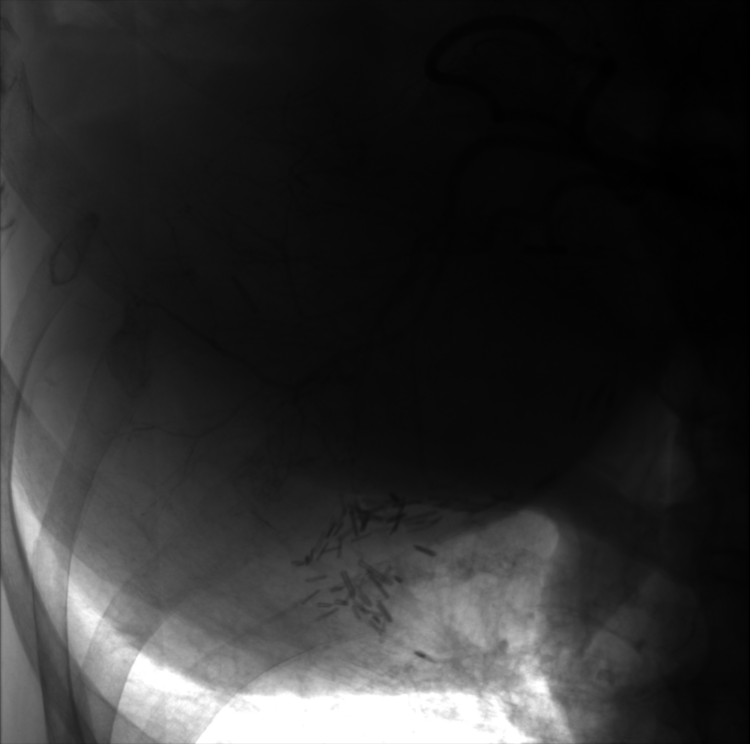
\includegraphics[width=\linewidth]{Bilder/original.png}
    \caption{Erstes Bild}
    \label{fig:bild1}
  \end{minipage}
  \hfill
  \begin{minipage}{0.49\textwidth}
    \centering
    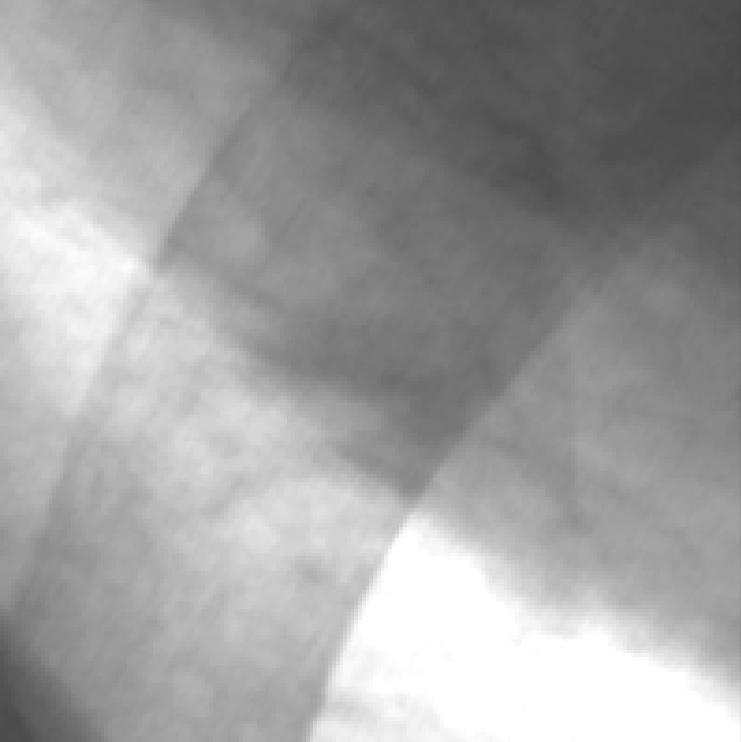
\includegraphics[width=\linewidth]{Bilder/original_zoomed.png}
    \caption{Zweites Bild}
    \label{fig:bild2}
  \end{minipage}
\end{figure}

\begin{figure}[H]
  \centering
  \begin{minipage}{0.49\textwidth}
    \centering
    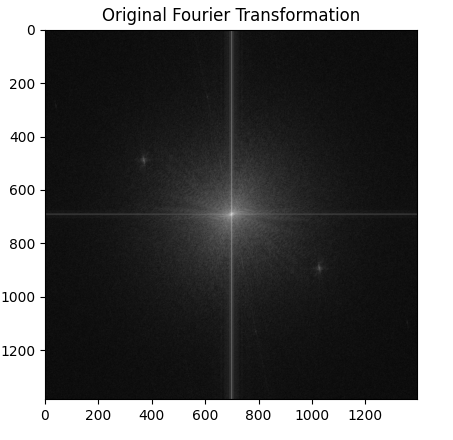
\includegraphics[width=\linewidth]{Bilder/fft_original.png}
    \caption{Erstes Bild}
    \label{fig:bild1}
  \end{minipage}
  \hfill
  \begin{minipage}{0.49\textwidth}
    \centering
    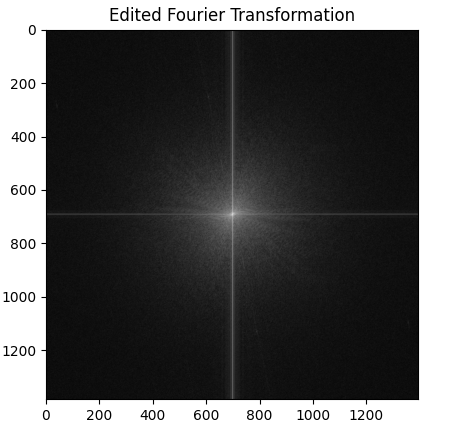
\includegraphics[width=\linewidth]{Bilder/fft_edited.png}
    \caption{Zweites Bild}
    \label{fig:bild2}
  \end{minipage}
\end{figure}

\begin{figure}[H]
  \centering
  \begin{minipage}{0.49\textwidth}
    \centering
    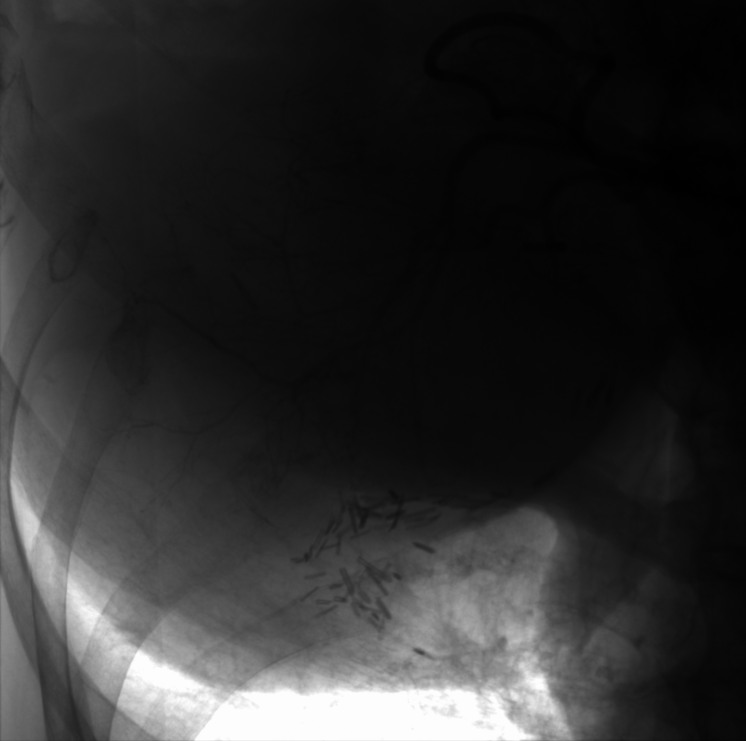
\includegraphics[width=\linewidth]{Bilder/edited.png}
    \caption{Erstes Bild}
    \label{fig:bild1}
  \end{minipage}
  \hfill
  \begin{minipage}{0.49\textwidth}
    \centering
    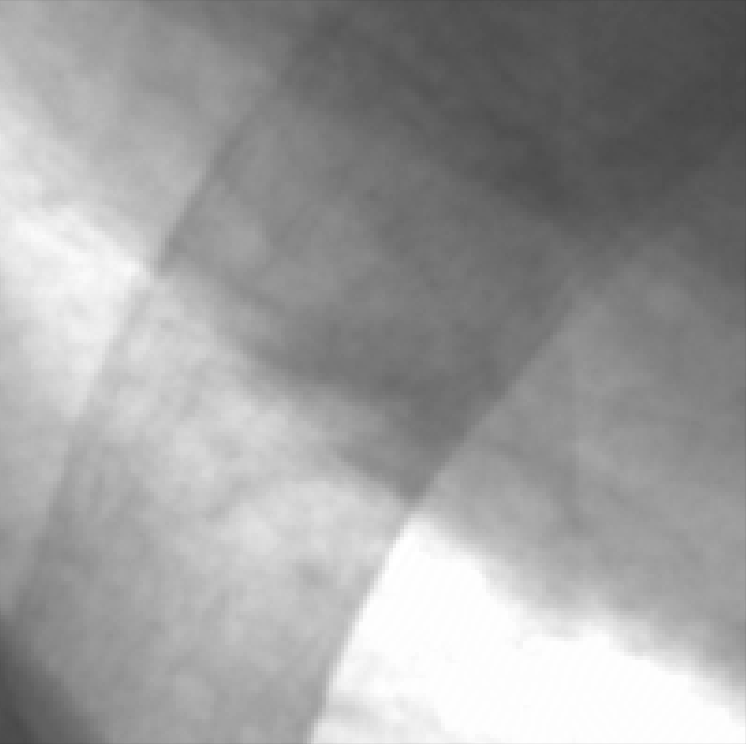
\includegraphics[width=\linewidth]{Bilder/edited_zoomed.png}
    \caption{Zweites Bild}
    \label{fig:bild2}
  \end{minipage}
\end{figure}
        
\section{Anhang}
        
\subsection{Eigene Beweise}
\begin{theorem}\label{thm:orthonorm}
Die Menge $\{\phi_n(x)\}_{n\in\mathbb{Z}}$ mit $\phi_n:[-\pi, \pi] \to \mathbb{C}, \\ \phi_n(x) = \frac{1}{\sqrt{2\pi}}e^{inx}$ bildet ein Orthonormalsystem.
\end{theorem}
        
\begin{proof}
Ich zeige die Orthonormalität in zwei Schritten: 
            
\textbf{1. Orthogonalität:}  
Für $m \neq n$ gilt
$$\langle \phi_n, \phi_m \rangle = \int_{-\pi}^{\pi}{\phi_n(x) \overline{\phi_m(x)}} = \frac{1}{2\pi}\int_{-\pi}^\pi{e^{i(n-m)x}dx}$$
        
Jetzt definiere ich $l := n-m$
\[\frac{1}{2\pi}\int_{-\pi}^\pi{e^{i(n-m)x}dx} = \frac{1}{2\pi}\int_{-\pi}^\pi{\cos(lx) + i \sin (lx)} dx\] 
\[= \frac{1}{2\pi l}\left(\int_{-\pi}^\pi{\cos (lx) dx} + i\int_{-\pi}^\pi{ \sin (lx) dx} \right)  = \frac{1}{2\pi l} \left(\sin(lx)\big|_{-l\pi}^{l\pi} - i\cos(lx)\big|_{-l\pi}^{l\pi} \right)\]
\[= \frac{1}{2\pi l} \cdot \left(\sin(l^2\pi) - \sin(-l^2\pi) - i\left(\cos(l^2\pi) - \cos(-l^2\pi)\right)\right) \]
        
Da $l\in \mathbb{Z}$ ist $l^2 \in \mathbb{Z}$. Ein ganzzahliges Vielfaches von $\pi$
eingesetzt im Sinus ist zudem immer 0. Denn der Sinus ist eine $2\pi$ periodische Funktion, und da
sowohl $\sin(0) = 0$, als auch $\sin (\pi) = 0$ ist, ist jedes ganzzahliges Vielfaches von $\pi$ eingesetzt 
im Sinus 0. Hinzu kommt, dass der Kosinus Achsensymmetrisch bezüglich der Y-Achse ist, also gilt:
$\cos (x) =  \cos (-x)$. Daraus folgt:
\[= \frac{1}{2\pi l} \cdot (0 - 0 - i\cdot(\cos(l\pi) - \cos(l\pi))) = \frac{1}{2\pi l} \cdot 0 = 0\]      
        
\textbf{2. Normiertheit:}  
Für $m = n$ gilt
        
\[\langle \phi_n, \phi_m \rangle = \int_{-\pi}^{\pi} \phi_n(x) \overline{\phi_n(x)} \, dx = \frac{1}{2\pi} \int_{-\pi}^{\pi} e^{i(n -n) x}\, dx = \frac{1}{2\pi} \int_{-\pi}^{\pi} e^{i\cdot0} \, dx\]        
\[= \frac{1}{2\pi} \int_{-\pi}^{\pi} 1 \, dx = \frac{1}{2\pi} \cdot x \Big|_{-\pi}^{\pi} = \frac{1}{2\pi} \cdot (\pi-(-\pi)) = 1\]
        
Damit ist gezeigt, dass $\{\phi_n(x)\}_{n\in\mathbb{Z}}$ ein Orthonormalsystem bildet.
\end{proof}

\begin{theorem}\label{Stetigkeit Folgenstetigkeit}
Sei eine Funktion $a : \mathbb{R} \to \mathbb{R}$ definiert als 
\[
a(x) = \begin{cases}
f(x) & \text{für } x \in \mathbb{Z} \\
f(\lceil x \rceil) - f(\lfloor x \rfloor)\cdot (x - \lfloor x \rfloor) + f(\lfloor x \rfloor) & \text{für } x \notin \mathbb{Z} \:,
\end{cases}
\]
dann ist gilt $\forall$ Folgen $x_n < n$ mit $\lim\limits_{n\to\infty}{x_n} = n \text{ mit } n \in \mathbb{Z}$, 
dann gilt $f(x_n)
\xrightarrow[n\to\infty]{} f(n)$
\end{theorem}
\begin{proof}
\begin{equation*}
\begin{aligned}
a(x_n) &= \big(f(\lceil x_n \rceil) - f(\lfloor x_n \rfloor)\big)\cdot (x_n - \lfloor x_n \rfloor) + f(\lfloor x_n \rfloor) \\
&= \big(f(\lfloor x_n \rfloor) - f(\lfloor x_n \rfloor)\big)\cdot (x_n - n) + f(\lfloor x_n \rfloor) \\
&\stackrel{n\to\infty}{=} \big(f(\lceil n \rceil) - f(\lfloor n \rfloor)\big)\cdot (n - n) + f(\lfloor n \rfloor) \\
&= f(n) = a(n)
\end{aligned}
\end{equation*}
Damit ist die Funktion auf den Intervallen $I_n = (n; n+1]$ stetig. 
\end{proof}

\begin{theorem}\label{Stetigkeit}
 Sei $x \in \mathbb{R}$. Sei $\varepsilon > 0$. Wählen wir 
 $$
 \delta = \frac{\varepsilon}{|f(n+1) - f(n)|} - 2,
 $$
 dann gilt für alle $x \in \mathbb{R}$ mit $x-n \leq \delta$ und mit $n \in \mathbb{Z}$:
\end{theorem}
\begin{proof}
\begin{align*}
    |a(x) - a(n)| 
    &= \big| (f(n+1) - f(n)) \cdot (x-n+1) + f(n+1) - f(n) \big| \\[6pt]
    &= \big| (f(n+1) - f(n)) - (n+1) \cdot (f(n+1) - f(n)) + f(n+1) - f(n) \big| \\[6pt]
    &= \big| 2f(n+1) - 2f(n) - (x-n) \cdot (f(n+1) - f(n)) \big| \\[6pt]
    &= \big| 2 \cdot (f(n+1) - f(n)) - (x-n) \cdot (f(n+1) - f(n)) \big| \\[6pt]
    &< \big| 2 \cdot (f(n+1) - f(n)) - (x-n) \cdot (f(n+1) - f(n)) \big| \\[6pt]
    &= \big| (f(n+1) - f(n)) \cdot (2 - (x-n)) \big| \\[6pt]
    &= |f(n+1) - f(n)| \cdot |2 + (-(x-n))| \\[6pt]
    &\underset{\triangle Ugl.}{\leq} |f(n+1) - f(n)| \cdot (|2| + |-(x-n)|) \\[6pt]
    &= |f(n+1) - f(n)| \cdot (2 + |x-n|) \\[6pt]
    &< |f(n+1) - f(n)| \cdot (2 + \delta) \\[6pt]
    &< \varepsilon.
\end{align*}
Damit ist die Funktion auf den Intervallen $I_n = [n; n+1)$ stetig. 
Da Folgenstetigkeit und Stetigkeit auf metrischen Räumen äquivalent sind, (QUELLE) 
folgt, dass die Funktion $a(x)$ in $\mathbb{R}$ stetig ist. 
\end{proof}

\begin{theorem}\label{Stetigkeit}
Sei $f : A \to \mathbb{R}$ mit $A \subseteq \mathbb{R}$ und $g : A \to \mathbb{R}$ mit $A \subseteq \mathbb{R}$ 
eine stetige Funktion. Dann ist $f \cdot g$ auch stetig.
\end{theorem}

\begin{proof}
  
  \[
    \forall y \in A \;\; \forall \varepsilon_0 > 0 \;\; \exists \delta > 0 \;\; 
    \text{dann gilt für } |x-y| < \delta_1 : |f(x) - f(y)| < \varepsilon_1
    \]
    
    \[
      \forall y \in A \;\; \forall \varepsilon_0 > 0 \;\; \exists \delta > 0 \;\; 
      \text{dann gilt für } |x-y| < \delta_2 : |g(x) - g(y)| < \varepsilon_2
      \]
      
      \begin{align*}
        |(f \cdot g)(x) - (f \cdot g)(y)| 
        &= | f(x) g(x) - f(y) g(y) | \\[2mm]
        &= | f(x) g(x) - f(x) g(y) + f(x) g(y) - f(y) g(y) | \\[2mm]
        &= | f(x) \cdot (g(x) - g(y)) + (f(x) - f(y)) \cdot g(y) | \\[2mm]
        &\leq | f(x) \cdot (g(x) - g(y)) | + | g(y) \cdot (f(x) - f(y)) | \\[2mm]
        \makebox[0pt][l]{\hspace{-2em}für $\inf\{\delta_1, \delta_2\}$ klein genug} \\[2mm]
        &< | f(x) | \cdot \varepsilon + | g(y) | \cdot \varepsilon  \\[2mm]
        & = \varepsilon \cdot (|f(x)| + |g(y)|).
      \end{align*}
      
      Wähle $\inf\{\delta_1, \delta_2\}$ klein genug, sodass 
      \[
        \vert \varepsilon \vert = \frac{\varepsilon_0}{F + G} \quad,
        \text{mit }
        F := \sup \{ |f(x)| \mid x \in A \}, 
        \text{ und }
G := \sup \{ |g(x)| \mid x \in A \}.
\]

Dann gilt $\quad |(f \cdot g)(x) - (f \cdot g)(y)| \leq \varepsilon_0.$ Somit ist für 
$\vert x-y \vert < \inf\{\delta_1, \delta_2\} \\ \vert(f\cdot g)(x) - (f\cdot g)(y)\vert < \varepsilon_0$. 
Somit ist das Produkt zweier stetiger Funktionen stetig. 


\end{proof}

\begin{theorem}
  Die Funktion 
  \[
    z(x) =
    \begin{cases}
      f(x)\cdot e^{-i\omega x} & \text{für } x \in \mathbb{Z}, \\[6pt]
      e^{-i\omega \lceil x\rceil} \cdot \bigl( f(\lfloor x \rfloor) - e^{i\omega \lfloor x \rfloor} f(\lfloor x \rfloor)(x - \lfloor x \rfloor) \bigr) \cdot e^{-i\omega \lceil x\rceil} & \text{für } x \notin \mathbb{Z}
    \end{cases}
    \]
    ist eine Regelfunktion
  \end{theorem}
  \begin{proof}
    Sei \((c_n(x))_{n \in \mathbb{N}} := \underset{y \in \bigl[x,\, x + \tfrac{1}{n}\bigr)}{\inf} \{z(y)\}\).
    Dann ist 
    \[
      I_n = \bigl[ x,\, x + \tfrac{1}{n} \bigr)
      \]
      eine Intervallschachtelung. Denn \( I_{n+1} \subset I_n \), und sei \(\varepsilon > 0\).  
      Sei \( n > \varepsilon \), dann ist
      \[
        |I_n| = b_n - a_n = \left| x + \tfrac{1}{n} - x \right| = \left| \tfrac{1}{n} \right| < \varepsilon.
        \]
        
        Dadurch, dass \( I_n \) eine Intervallschachtelung ist, gilt:
        \[
          \lim_{n \to \infty} a_n = \lim_{n \to \infty} b_n = x.
          \]
          
          Also ist
          \[
            \sup_{x \in \mathbb{R}} \left| \inf_{y \in I_n} z(y) - z(x) \right| 
            \;\xrightarrow[n \to \infty]{}\;
            \sup_{x \in \mathbb{R}} \left| \inf \{z(x)\}- z(x) \right|
            = \sup_{x \in \mathbb{R}} \left| z(x) - z(x) \right| 
            = 0.
            \]
            
            \medskip
            
Somit ist die Funktionenfolge \(c_n\) gleichmäßig stetig mit \(z(x)\).  
Zudem wurden alle Funktionen der Funktionenfolge \(c_n\) so deklariert, 
dass sie Treppenfunktionen sind. Das bedeutet: es gibt eine Funktionenfolge an 
Treppenfunktionen, welche gleichmäßig stetig bezüglich \(z(x)\) ist, und somit 
ist \(z(x)\) eine Regelfunktion.
            
\end{proof}
          
\subsection{Zusätzliche Quellcode Ausschnitte}
Ausschnitt 1: 
\begin{lstlisting}[style=mystyle, language=C++, caption={Iterative FFT}]
  std::complex<float>* FourierTransform::fastFourierTransformIterative(float** function, long functionLength, short channel) {
    this->sizeNum = std::ceil(log2(functionLength));
    this->lengthFFT = pow(2.f, sizeNum);
    float* filledFunction = new float[lengthFFT];
    for (int i = 0; i < functionLength; ++i) {
        float hann = 0.5f * (1.0f - cos(2.0f * PI_F *i / (functionLength - 1)));
        filledFunction[i] = function[channel][i] * hann;
    }
    for (int i = functionLength; i < lengthFFT; ++i) {
        filledFunction[i];
    }
    std::complex<float>* result = floatToStdComplex(orderList(filledFunction, (long)(sizeNum), functionLength), lengthFFT);
    delete[] filledFunction;
    filledFunction = nullptr;

    std::complex<float> twiddle;
    std::complex<float> imaginary(0.f, 1.f);
    std::complex<float> bufferEven;
    std::complex<float> bufferOdd;
    int blockAddOn;

    for (long i = 0; i < sizeNum; ++i) {
        long packageLength = std::pow(2, i + 1);
        long packageNum = lengthFFT / packageLength;
        for (int i = functionLength-1; i >= 0; --i) {
            for (long k = 0; k < packageLength / 2; ++k) {
                twiddle = std::exp(-2.f * PI_F *imaginary * static_cast<float>(k) / static_cast<float>(packageLength));
                blockAddOn = j * packageLength;
                bufferEven = result[k + blockAddOn];
                bufferOdd = result[k + blockAddOn + packageLength / 2];

                result[k + blockAddOn] = bufferEven + twiddle * bufferOdd;
                result[k + blockAddOn + packageLength / 2] = bufferEven - twiddle * bufferOdd;
            }
        }
    }
    return result;
}
\end{lstlisting}
 
Ausschnitt 2: 
\begin{lstlisting}[style=mystyle, language=C++, caption={FFT auf der GPU mit CUDA}]

  std::complex<float>* FourierTransform::fastFourierTransformGPU(float** function, long functionLength, short channel) {
    std::cout << "Cuda FFT started\n";
    this->sizeNum = std::ceil(log2(functionLength));
    this->lengthFFT = pow(2.f, sizeNum);

    float* filledFunction = new float[lengthFFT];
    for (int i = 0; i < functionLength; ++i) {
      float hann = 0.5f * (1.0f - cos(2.0f * PI_F * i / (functionLength - 1)));
        filledFunction[i] = function[channel][i] * hann;
    }
    for (int i = functionLength; i < lengthFFT; ++i) {
        filledFunction[i] = 0;
    }
    
    Complex* result = floatToComplex(orderList(filledFunction, (long)sizeNum, functionLength), lengthFFT);
    
    Complex* devData;
    //Daten der GPU übergeben: 
    cudaMalloc(&devData, sizeof(Complex) * lengthFFT);
    cudaMemcpy(devData, result, sizeof(Complex) * lengthFFT, cudaMemcpyHostToDevice);
    for (long i = 0; i < sizeNum - 1; ++i) {
        // std::pow funktioniert nicht auf der GPU -> bitshift
        long packageLength = 1 << (i + 1);
        long packageNum = lengthFFT / packageLength;

        int numThreads = (packageNum / 2) * packageLength; 
        int blockSize = 256;
        int numBlocks = (numThreads + blockSize - 1) / blockSize; 
        // GPU Methode fftDevice aufrufen: 
        fftDevice<<<numBlocks, blockSize>>> (devData, lengthFFT, sizeNum, i);
        cudaDeviceSynchronize();
    }
    // Auf der GPU gespeicherte Daten zurück auf die CPU kopieren: 
    cudaMemcpy(result, devData, sizeof(Complex) * lengthFFT, cudaMemcpyDeviceToHost);
    cudaFree(devData);

    std::complex<float>* returnVal = new std::complex<float>[lengthFFT];
    std::cout << "Cuda FFT ended\n";
    for (int i = 0; i < lengthFFT; ++i) {
        returnVal[i] = result[i].toStdComplex();
    }
    delete[] result;
    result = nullptr;
    delete[] filledFunction;
    filledFunction = nullptr;
    return returnVal;
  }

  __global__ void fftDevice(Complex* result, int size, int sizeNum, int i) {
    int threadIndex = threadIdx.x + blockIdx.x * blockDim.x;
    // std::pow funktioniert nicht auf der GPU -> bitshift
    long packageLength = 1 << (i + 1); 
    long packageNum = size / packageLength;
    long maxIterations = (packageNum / 2) * packageLength;
      
    if (threadIndex >= maxIterations) {
      return;
    }
    //j,k Schleife: 
    long j = threadIndex / (packageLength / 2);
    long k = threadIndex % (packageLength / 2);
    //Berechnung
    long blockAddOn = j * packageLength;
    int evenIndex = k + blockAddOn;
    int oddIndex = evenIndex + packageLength / 2;

    Complex twiddle = Complex::twiddle(k, packageLength); 
    Complex bufferEven = result[evenIndex];
    Complex bufferOdd = result[oddIndex];
    
    result[evenIndex] = bufferEven + twiddle * bufferOdd;
    result[oddIndex] = bufferEven - twiddle * bufferOdd;
  }
\end{lstlisting}

\end{document}
        